\documentclass{beamer}
%
% Choose how your presentation looks.
%
% For more themes, color themes and font themes, see:
% http://deic.uab.es/~iblanes/beamer_gallery/index_by_theme.html
%

\mode<presentation>
{
  \usetheme{Madrid}      % or try Darmstadt, Madrid, Warsaw, ...
  \usecolortheme{beaver} % or try albatross, beaver, crane, ...
  \usefonttheme{default}  % or try serif, structurebold, ...
  \setbeamertemplate{navigation symbols}{}
  \setbeamertemplate{caption}[numbered]
} 
\usepackage{pifont}
\usepackage[bookmarks]{hyperref}
\usepackage[backend=bibtex]{biblatex}
\usepackage{braket}
\addbibresource{bibliography.bib}
\newtheorem*{remark}{Remark}
\usepackage[english]{babel}
\usepackage[utf8x]{inputenc}
\usebackgroundtemplate{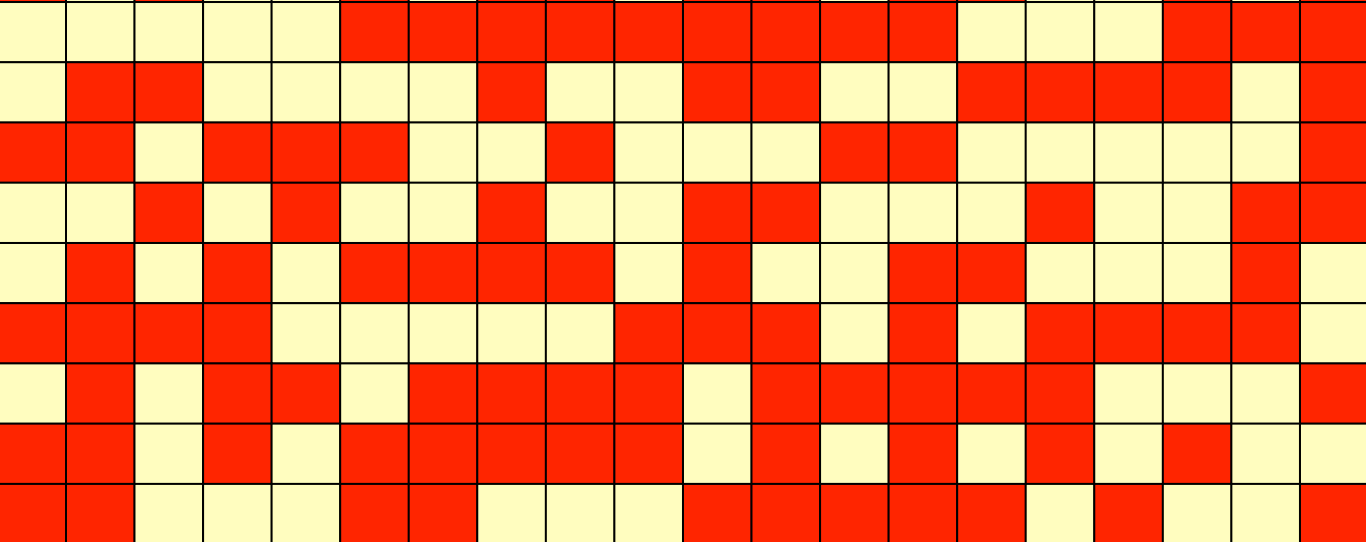
\includegraphics[width=\paperwidth]{Pic/Intro_pict.png}}
\title[AMS project]{ Stationary states of opinion diffusion}
\subtitle{Project for the exam: AMS (DSE)}
\author{Paola Serra and Marzio De Corato }
\date{\today}

\begin{document}

\begin{frame}
\vspace{+4 cm}  \titlepage
\end{frame}

\usebackgroundtemplate{ } 

% Uncomment these lines for an automatically generated outline.
%\begin{frame}{Outline}
%\setcounter{tocdepth}{1}
%\begin{center}
%  \tableofcontents
%\end{center}
%\end{frame}





\begin{frame}{}
\begin{center}
{\Huge Theoretical Framework}
\end{center}
\end{frame}


\section{Statistical Mechanics}

\begin{frame}{}
\begin{center}
{\Huge Statistical Mechanics}
\end{center}
\begin{center}
\textit{“Ludwig Boltzmann, who spent much of his life studying statistical mechanics, died in 1906, by his own hand. Paul Ehrenfest, carrying on the work, died similarly in 1933. Now it is our turn to study statistical mechanics.” States of Matter (1975), by David L. Goodstein}
\end{center}
\end{frame}

\begin{frame}{Concepts of statistical mechanics: aim \cite{peliti2011statistical}}
\begin{center}
\textbf{Aim} To predict the macroscopic properties of systems on the basis of their microscopic structure. This connection between these two scales is performed with statistical methods
\end{center}
\end{frame}

\begin{frame}{Concepts of statistical mechanics: entropy and temperature \cite{frenkel2001understanding}}
\begin{itemize}
\item Consider a system with total energy E that is composed by two subsystems (with energy $E_{1}$ and $E_{2}$ that can exchange only energy - canonical ensemble) 
\item There are many way in which the energy can distribute in the two systems with the constrain $E=E_{1}+E_{2}$
\item In particular given the energy $E_{1}$ the total number of degenerate states is $\Omega_{1}(E_{1})\times\Omega_{1}(E_{2}) $
\item We would have a measure of the degeneracy of the system that is additive, therefore 
\end{itemize}
\begin{equation*}
\ln\Omega(E_{1},E-E_{1})=\ln\Omega_{1}(E_{1})+\ln\Omega_{2}(E-E_{1})
\end{equation*}
\begin{itemize}
\item Every energy state of the total system is equal likely. Therefore the most probable state is the one that maximizes $\ln \Omega(E_{1},E-E_{1})$
\end{itemize}
\begin{equation*}
\left( \frac{\partial \ln \Omega(E_{1},E-E_{1})}{\partial E_{1}} \right)_{N,V,E}=0
\end{equation*}
\end{frame}


\begin{frame}{Concepts of statistical mechanics: entropy and temperature \cite{frenkel2001understanding}}
\begin{itemize}
\item The previous statement is equal to the following one
\end{itemize}
\begin{equation*}
\left( \frac{\partial \ln \Omega(E_{1})}{\partial E_{1}} \right)_{N1,V1}=\left( \frac{\partial \ln \Omega(E_{2})}{\partial E_{2}} \right)_{N2,V2}
\end{equation*}
\begin{itemize}
\item Introducing the following notation
\end{itemize}
\begin{equation*}
\beta\equiv\left( \frac{\partial \ln \Omega(E_{1})}{\partial E_{1}} \right)_{N1,V1}
\end{equation*}
\begin{itemize}
\item And introducing the concept of entropy 
\end{itemize}
\begin{equation*}
S(N,V,E)\equiv k_{b}ln\Omega(N,V,E)
\end{equation*}
We have the definition of thermodynamic temperature 
\begin{equation*}
\frac{1}{T}=\left( \dfrac{\partial S}{\partial E} \right)_{V,N}
\end{equation*}
\begin{equation*}
\equiv\dfrac{1}{k_{b}T}
\end{equation*}
\end{frame}

\begin{frame}{Concepts of statistical mechanics: entropy and temperature \cite{frenkel2001understanding}}
\begin{itemize}
\item So we have proof the at the equilibrium, the configuration with maximum entropy, the temperature of the two sub-systems is equal 
\end{itemize}
\begin{equation*}
T_{1}=T_{2}
\end{equation*}
\end{frame}



\begin{frame}{Concepts of statistical mechanics: entropy and temperature \cite{frenkel2001understanding}}
\begin{itemize}
\item Given that the system 1 is in the state $E_{1}$ the second system have energy $E-E_{i}$. Therefore the degeneracy of the second system is equal to $\Omega(E-E_{i})$
\item Thus the probability of 1 to be in the state i will be 
\end{itemize}

\begin{equation*}
P_{i}=\dfrac{\Omega(E-E_{i})}{\sum_{j}\Omega(E-E_{j})}
\end{equation*}
\begin{itemize}

\item Expanding around $E_{i}=0$
\end{itemize}
\begin{equation*}
\ln\Omega_{B}(E-E_{i})=\ln\Omega_{B}(E)-E_{i}\frac{\partial\log\Omega_{B}(E)}{\partial E}+O(1/E)
\end{equation*}
\begin{equation*}
\ln\Omega_{B}(E-E_{i})=\ln\Omega_{B}(E)-\dfrac{E_{i}}{k_{b}T}+O(1/E)
\end{equation*}
\begin{equation*}
P_{i}=\dfrac{\exp(-E_{i}/k_{b}T)}{\sum_{j}\exp(-E_{j}/k_{b}T)}
\end{equation*}


\end{frame}


\begin{frame}{Concepts of statistical mechanics: phase portrait \cite{peliti2011statistical}}
 \begin{center}
     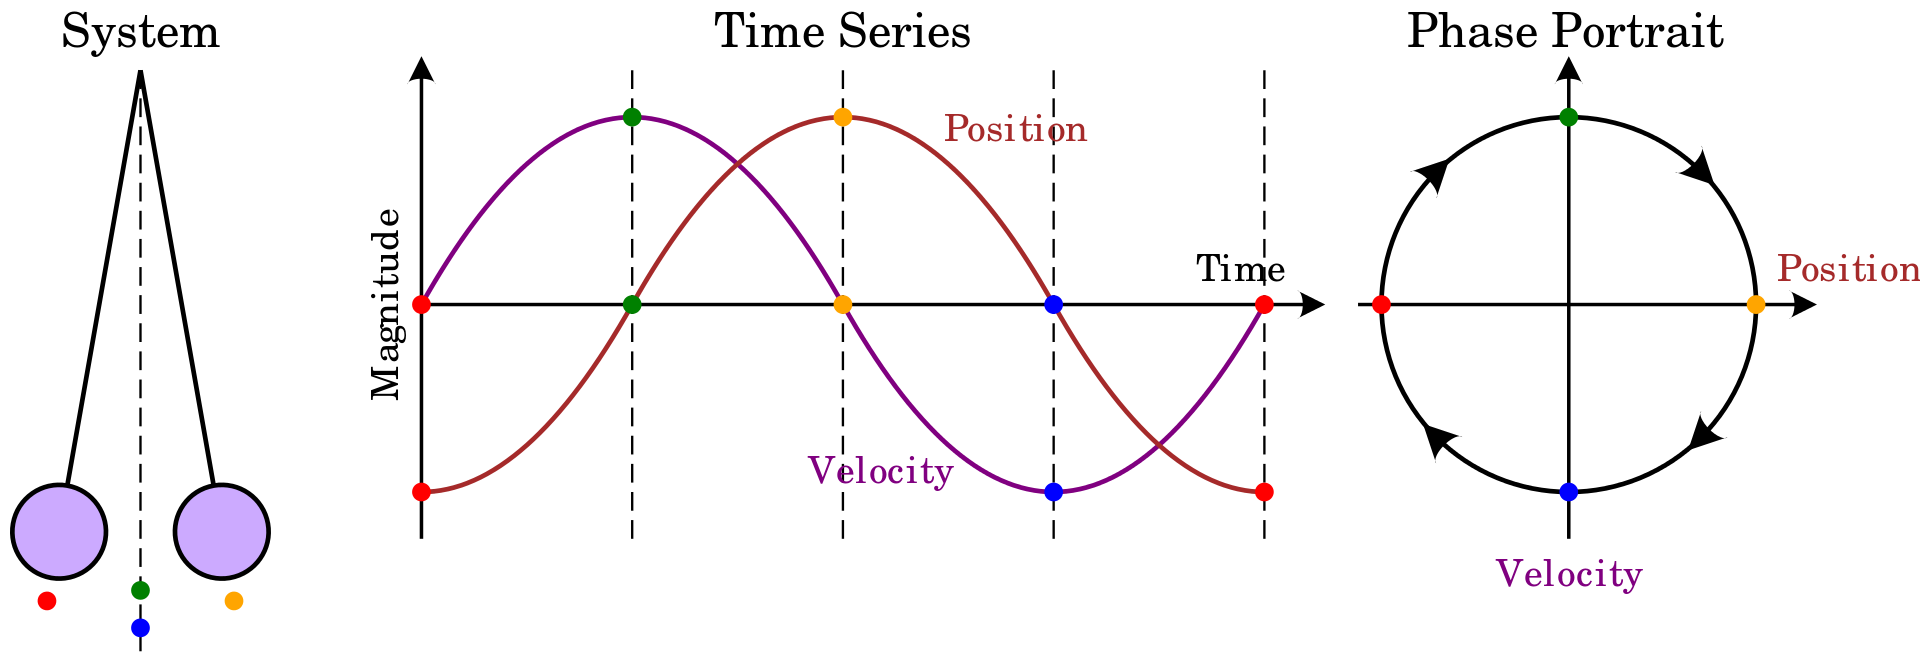
\includegraphics[width=0.7\textwidth]{Pic/Pendulum_phase_portrait_illustration.png}
\end{center}
\begin{center}
Image taken from \cite{PBC}
\end{center}




\end{frame}


\begin{frame}{Concepts of statistical mechanics: ensemble \cite{peliti2011statistical}}

\begin{itemize}
\item \textbf{Statistical ensemble}: a large number of virtual copies of a system ; each of them  is a possible state of the real system (epistemic probability) . It is the formalization of a repeated experiment proposed by Gibbs (empirical probability)
\item\textbf{ Microcanical ensamble:} $p=1/W$ $W$ is the number of microstates
\item \textbf{Canonical ensamble:} $p=\frac{1}{Z}\exp\left(-\frac{E}{kT}\right)$ where $Z=\sum_{i}\exp\left(\dfrac{-E_{i}}{k_{b}T}\right)$
\end{itemize}
\begin{equation}
\left\langle A(x) \right\rangle=\dfrac{1}{Z}\int dx_{s}A(x_{s})exp\left[ -\frac{H^{(S)}(x_{s})}{k_{b}T} \right]
\end{equation}

\begin{equation}
Z=\int dx_{s}exp\left[  -\frac{H^{S}(x_{s})}{k_{b}T}  \right]
\end{equation}

\begin{equation}
\left\langle H(x)^{2} \right\rangle-\left\langle H(x) \right\rangle^{2}=k_{b}T^{2}C
\end{equation}


\end{frame}





\section{Ising model}

\begin{frame}{}
\begin{center}
{\Huge Ising Model}
\end{center}
\end{frame}


\begin{frame}{Ising model \cite{mackay2003information,slides}}
\begin{itemize}
\item An array of atoms that can take states $\pm 1$. The energy of the system is given by $E(\textbf{x},J,H)= - \left[\dfrac{1}{2}\sum_{m,n}J_{mn}x_{m}x_{n}+\sum_{n}Hx_{n} \right]$ where J is the coupling constant between two neighbour sites, and H is an external field. 
\item The probability of the system to be in the state x is given by $p(x|\beta,J,H)=\frac{1}{Z(\beta,J,H)}\exp[-\beta E(x,J,H)]$ (canonical ensemble) where $\beta=1/k_{b}T\quad Z(\beta,J,H)=\sum_{x}exp\left[-\beta E(x,J,H)\right]$
\item It is useful to characterize the order level of a lattice (macroscopic) with the (spatial) correlation functions (whose input are microscopic quantities). In particular, for the Ising model, these are given by the following expression (with $H=0$)
\end{itemize}


\begin{equation*}
g(m)=\frac{\left\langle \sigma_{i}\sigma_{i+m}  \right\rangle - \left\langle \sigma_{i} \right\rangle \left\langle \sigma_{i+m} \right\rangle  }{1- \left\langle \sigma_{i} \right\rangle \left\langle \sigma_{i+m} \right\rangle }=\left\langle \sigma_{i}\sigma_{i+m}  \right\rangle $ 
\end{equation*}

\end{frame}

\section{Numerical simulation}

\begin{frame}{}
\begin{center}
{\Huge Numerical simulations}
\end{center}
\begin{center}
\textit{“Never make a calculation until you know the answer. Make an estimate before every calculation, try a simple physical argument (symmetry! invariance! conservation!) before every derivation, guess the answer to every paradox and puzzle. Courage: No one else needs to know what the guess is. Therefore make it quickly, by instinct. A right guess reinforces this instinct. A wrong guess brings the refreshment of surprise. In either case life as a spacetime expert, however long, is more fun!” John Archibald Wheeler }
\end{center}
\end{frame}


\begin{frame}{Numerical simulation \cite{peliti2011statistical}}
\begin{itemize}
\item\textbf{Molecular dynamics:} the equation of motion are solved numerically PROS: information of both the dynamical and static properties of the system are explored 
\item\textbf{Monte Carlo:} a fictitious evolution process of the system is solved in order to get the equilibrium distribution PROS  1) also the systems whose dynamics is not defined can be explored 2) a fictitious dynamics can be considered in order to reach the equilibrium faster 
\end{itemize}
\end{frame}


\begin{frame} {Monte Carlo method \cite{frenkel2001understanding}}
 \begin{center}
     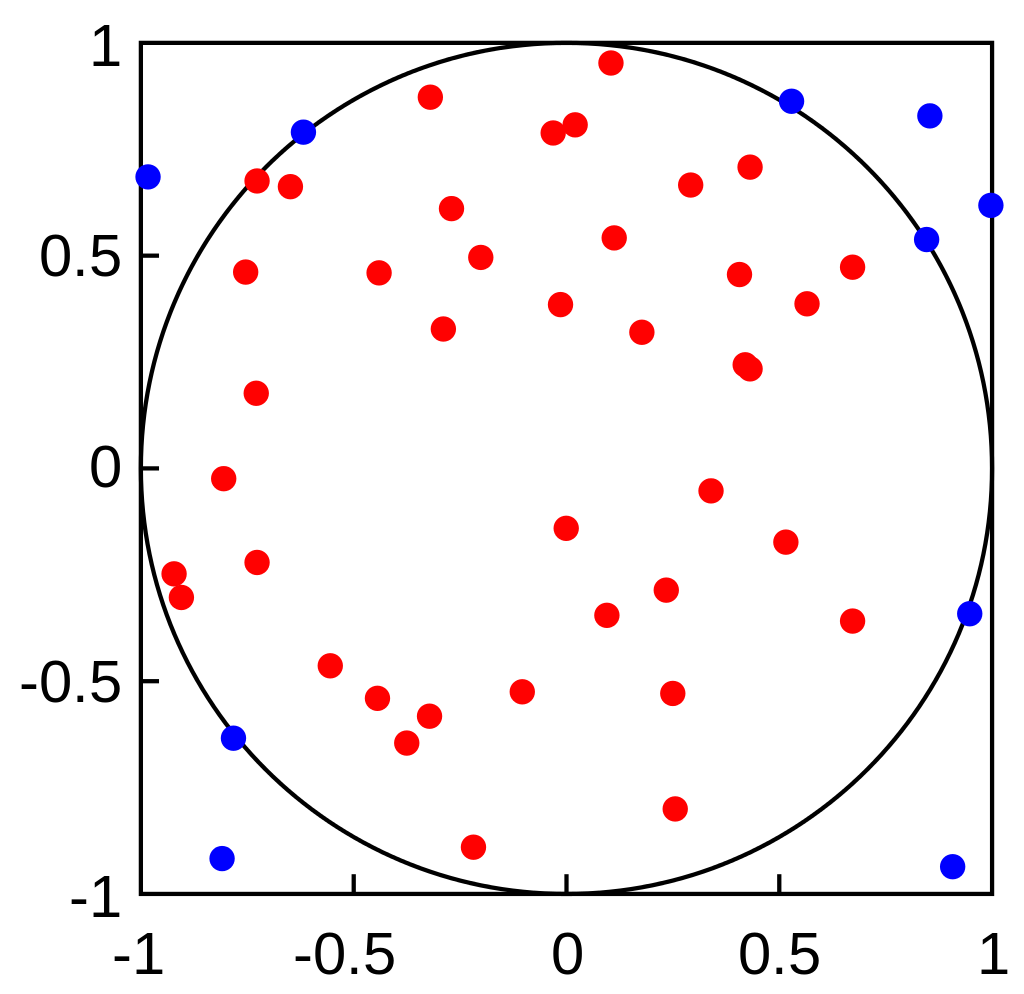
\includegraphics[width=0.5\textwidth]{Pic/MonteCarloIntegrationCircle.png}
\end{center}
 \begin{center}
Image taken from \cite{PBC}
\end{center}
\end{frame}




\begin{frame}{Monte Carlo method \cite{frenkel2001understanding}}
\begin{itemize}
\item Lets consider the generic integral $I=\int^{b}_{a}dx\;f(x)$
\item This can be recast in the following form  $I=\int^{1}_{0}dx\;w(x)\dfrac{f(x)}{w(x)}$
\item If w(x) is the derivative of u(x) (non-decreasing,non negative) we have $I=\int^{1}_{0}du\;\dfrac{f[x(u)]}{w[x(u)]}$
\item If one considers L random values of u uniformely distributed in the interval [0,1] we have $I\approx\dfrac{1}{L}\sum_{i=1}^{L}\dfrac{f[x(u)}{w[x(x)]}$
 \item The choice of w is crucial since $\sigma=\dfrac{1}{L}\left[\left\langle\left(\dfrac{f}{w}\right)^{2}\right\rangle-  \left\langle\dfrac{f}{w}\right\rangle^{2}\right]$
 \item Brute Force $f=10^{-260}$ and $\sigma=\dfrac{1}{Lf}$...is not a good idea
 \item PROBLEM: we do not know the form of the denominator (if we know it we do not need the Monte Carlo method)


\end{itemize}
\end{frame}


\begin{frame} {Monte Carlo method \cite{peliti2011statistical}}

 \begin{center}
     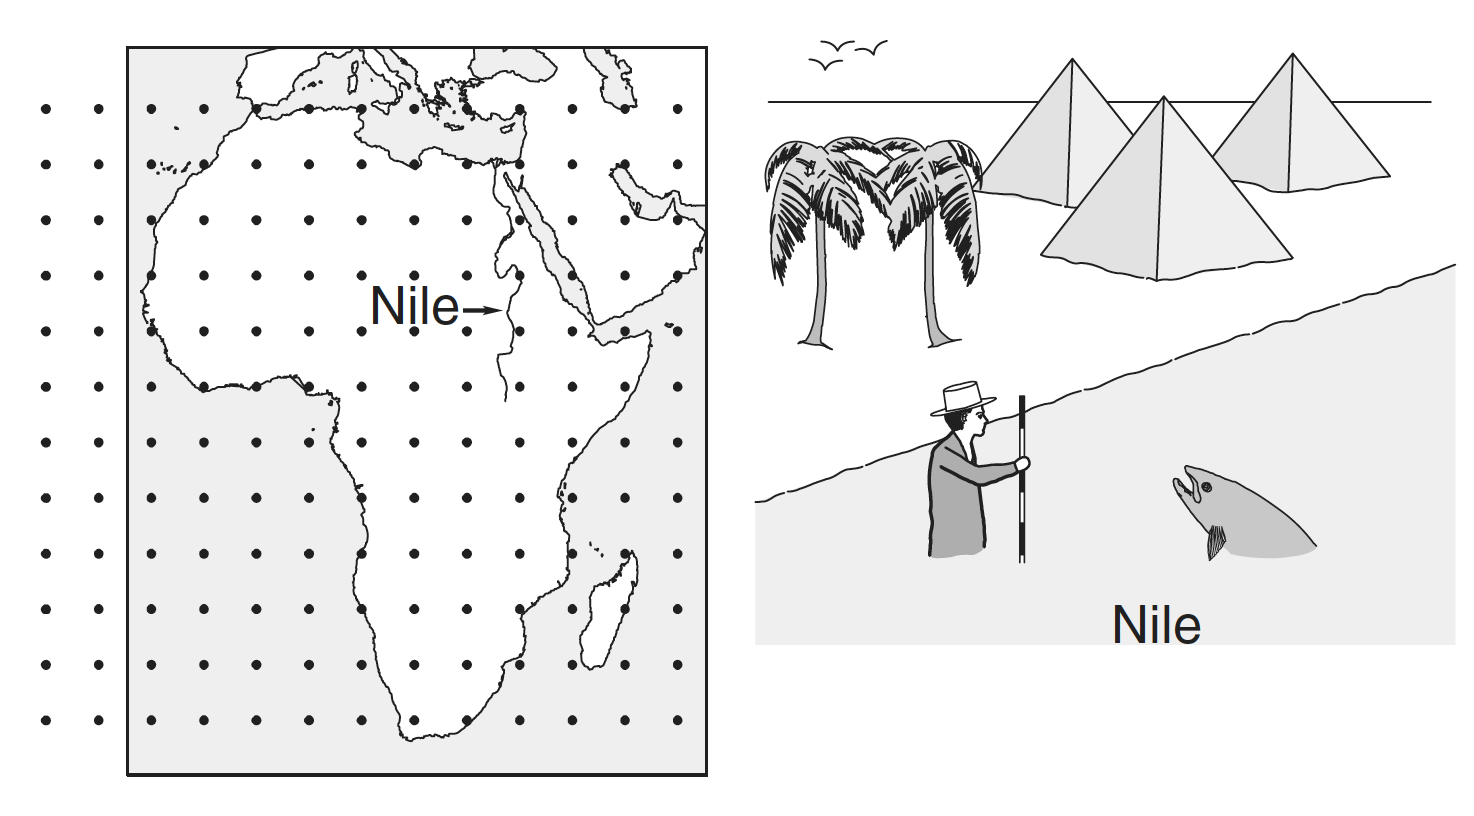
\includegraphics[width=0.7\textwidth]{Pic/Pic_river.png}
\end{center}
 \begin{center}
Image taken from \cite{frenkel2001understanding}
\end{center}
\end{frame}


\begin{frame}{Monte Carlo method: Metropolis idea \cite{frenkel2001understanding}}


\begin{equation}
\left\langle A \right\rangle=\dfrac{\int d\textbf{r}^{N}\exp\left[ -\beta E(\textbf{r}^{N}) \right]A(r^{N})}{\int d\textbf{r}^{N}\exp\left[ -\beta E(\textbf{r}^{N}) \right]}
\end{equation}

\begin{itemize}
\item We have a ratio between two integrals, therefore what we need to sample is the ratio and not the integrals alone
\item The probability density is $N(r^{N})=\exp\left[-\beta E(\textbf{r}^{N}) \right]/Z$
\item Metropolis idea: randomly generate points with this last probability distribution. In this case we have $\left\langle A \right\rangle \approx 1/L\sum_{i=1}^{L}n_{i}A(\textbf{r}_{i}^{N})$

\end{itemize}
\end{frame}


\begin{frame}{Monte Carlo method: Metropolis idea \cite{frenkel2001understanding}}

\begin{itemize}

\item How the points are generated ? With a Boltzmann weighted Markov chain
\item $\pi(old \rightarrow new) = \alpha (old \rightarrow new) \times acc(old \rightarrow new) $ where $\pi$ is the transition probability element from the old state to the new state,$\alpha$ is the matrix element of Markov Chain and acc is the acceptance ratio. 
\item Detailed balance condition at the equilibrium $N(old)\pi(old \rightarrow new)= N(new)\pi(new \rightarrow old) $ 
\item With a symmetric Markov transition matrix we have $N(old)\times acc(old\rightarrow new) = N(new) \times acc(new\rightarrow old)$
\item Therefore we have 
\end{itemize}

\begin{equation}
\frac{acc(old \rightarrow new)}{acc(new \rightarrow old)}=\dfrac{N(n)}{N(o)}=\exp\left[ -\beta \left( E(new)-E(old) \right) \right]
\end{equation}
\begin{itemize}
\item THE Z TERM IS NO MORE PRESENT ! We have only the difference between the two energies !!!
\end{itemize}


\end{frame}


\begin{frame}{Monte Carlo method: Metropolis idea \cite{frenkel2001understanding}}

\begin{equation*}
acc(old \rightarrow new) = \begin{cases} N(new)/N(old)\quad N(new) < N(old) \\
1 \quad N(new) \geq N(old)  \end{cases}
\end{equation*}
\begin{itemize}
Therefore the overall transition probabilities are given by 
\end{itemize}
\begin{equation*}
\begin{split}
\pi(old \rightarrow new) &= \begin{cases} \alpha(old \rightarrow new)\quad N(new) \geq N(old) \\
\alpha(old \rightarrow new)  \left[  N(new)/N(old) \right] \quad N(new) < N(old) \end{cases} \\
\pi(old \rightarrow new) & = 1-\sum_{new\neq old} \pi(old\rightarrow new)
\end{split}
\end{equation*}
\begin{itemize}
\item In practice for each move a random number is generated from the uniform distribution between the interval $[0,1]$, since $acc(old \rightarrow new) = \exp\left[ -\beta \left( E(new)-E(old) \right)\right] < 1 $. The move is accepted if the random number is lower than $acc(old \rightarrow new)$
\item $\pi(old \rightarrow new)$ should be ergodic
\end{itemize}


\end{frame}






\section{Goals and methods}

\begin{frame}
\begin{center}
{\Huge Goals and methods}
\end{center}
\end{frame}

\begin{frame}{Goals and methods}
\begin{itemize}
\item Reproduce the main result for a 2D anti ferromagnetic lattice $(J=-1)$ with no external magnetic field $(H=0)$ with the montecarlo-metropolis
\item  Once checked that the script provide the correct results apply it to a lattice $(J=+1)$.  In this case the spins represent an opinion and the sites people.  The goal is to find the stationary states (at $T=0$ and $T\neq0$)
\item Introduce in the lattice some blocks that never change their status.  These islands represent groups that never change mind and only diffuse their ideas.  (at $T=0$ and $T\neq0$)
\end{itemize}
\end{frame}

\section{Results}

\begin{frame}
\begin{center}
{\Huge Results}
\end{center}
\end{frame}

\begin{frame}{Simulation features}
\begin{itemize}
\item 10x10 lattice 
\item Periodic boundary conditions $\rightarrow$ the topology of a torus (genus equal to 1) 
\item 6000 steps 
\end{itemize}
\begin{columns}
\begin{column}{0.5\textwidth}
    \begin{center}
     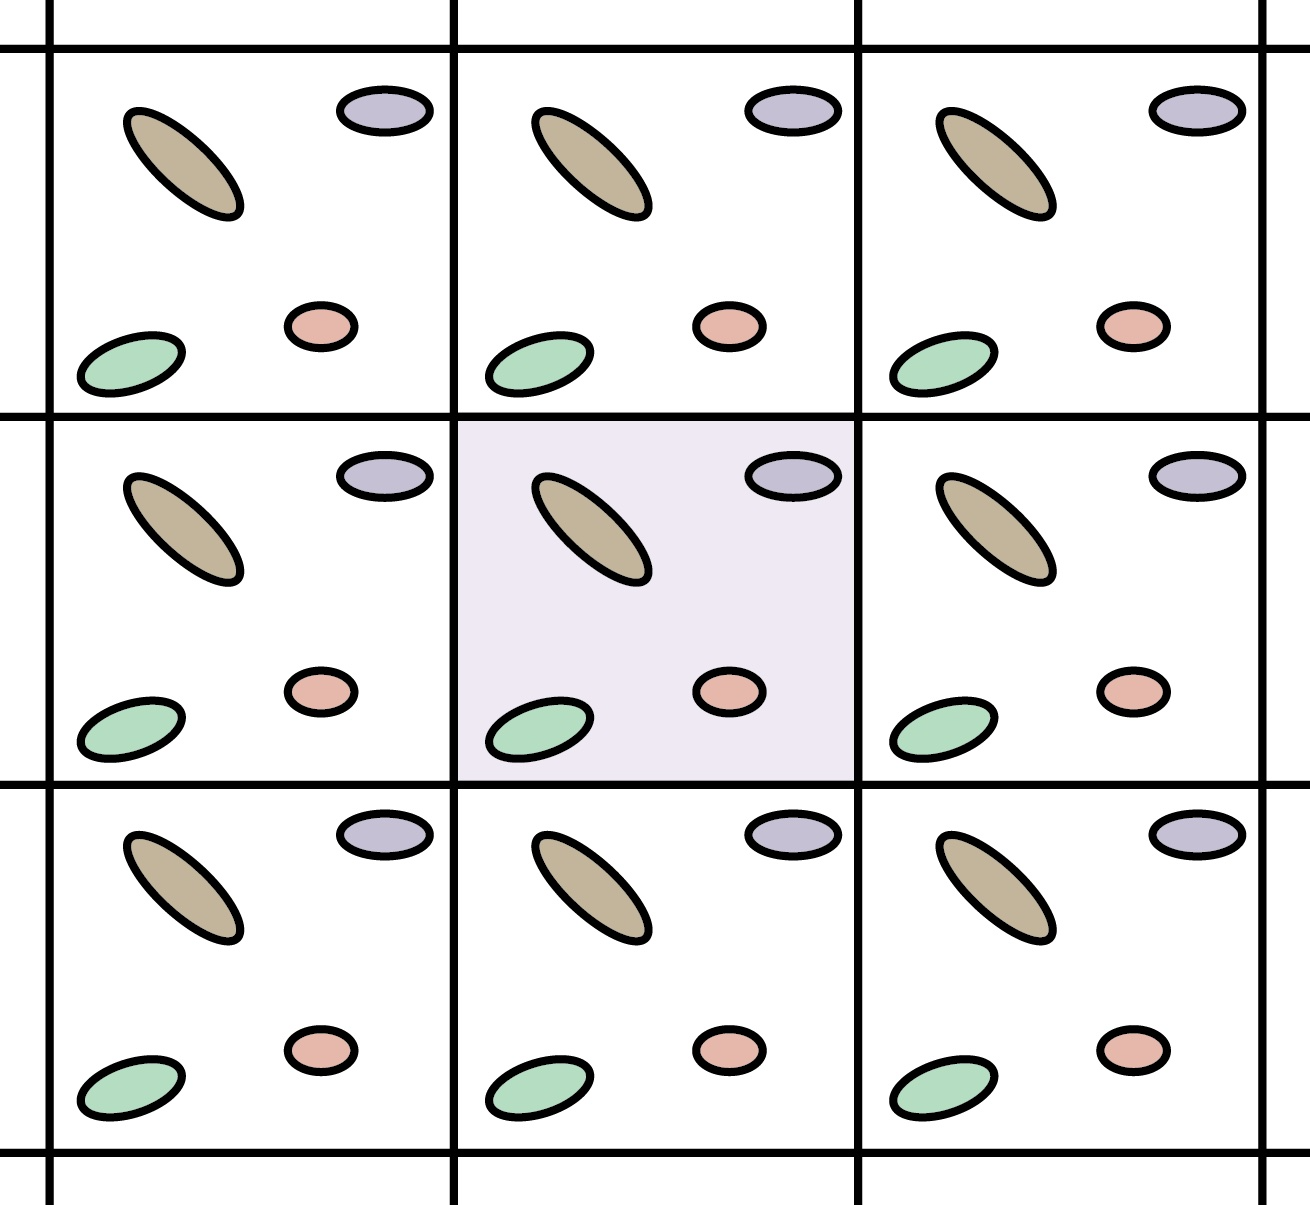
\includegraphics[width=0.7\textwidth]{Pic/PBC.png}
      \end{center}
      \begin{center}
          Image taken from \cite{PBC}
     \end{center}
\end{column}
\begin{column}{0.5\textwidth}

    \begin{center}
     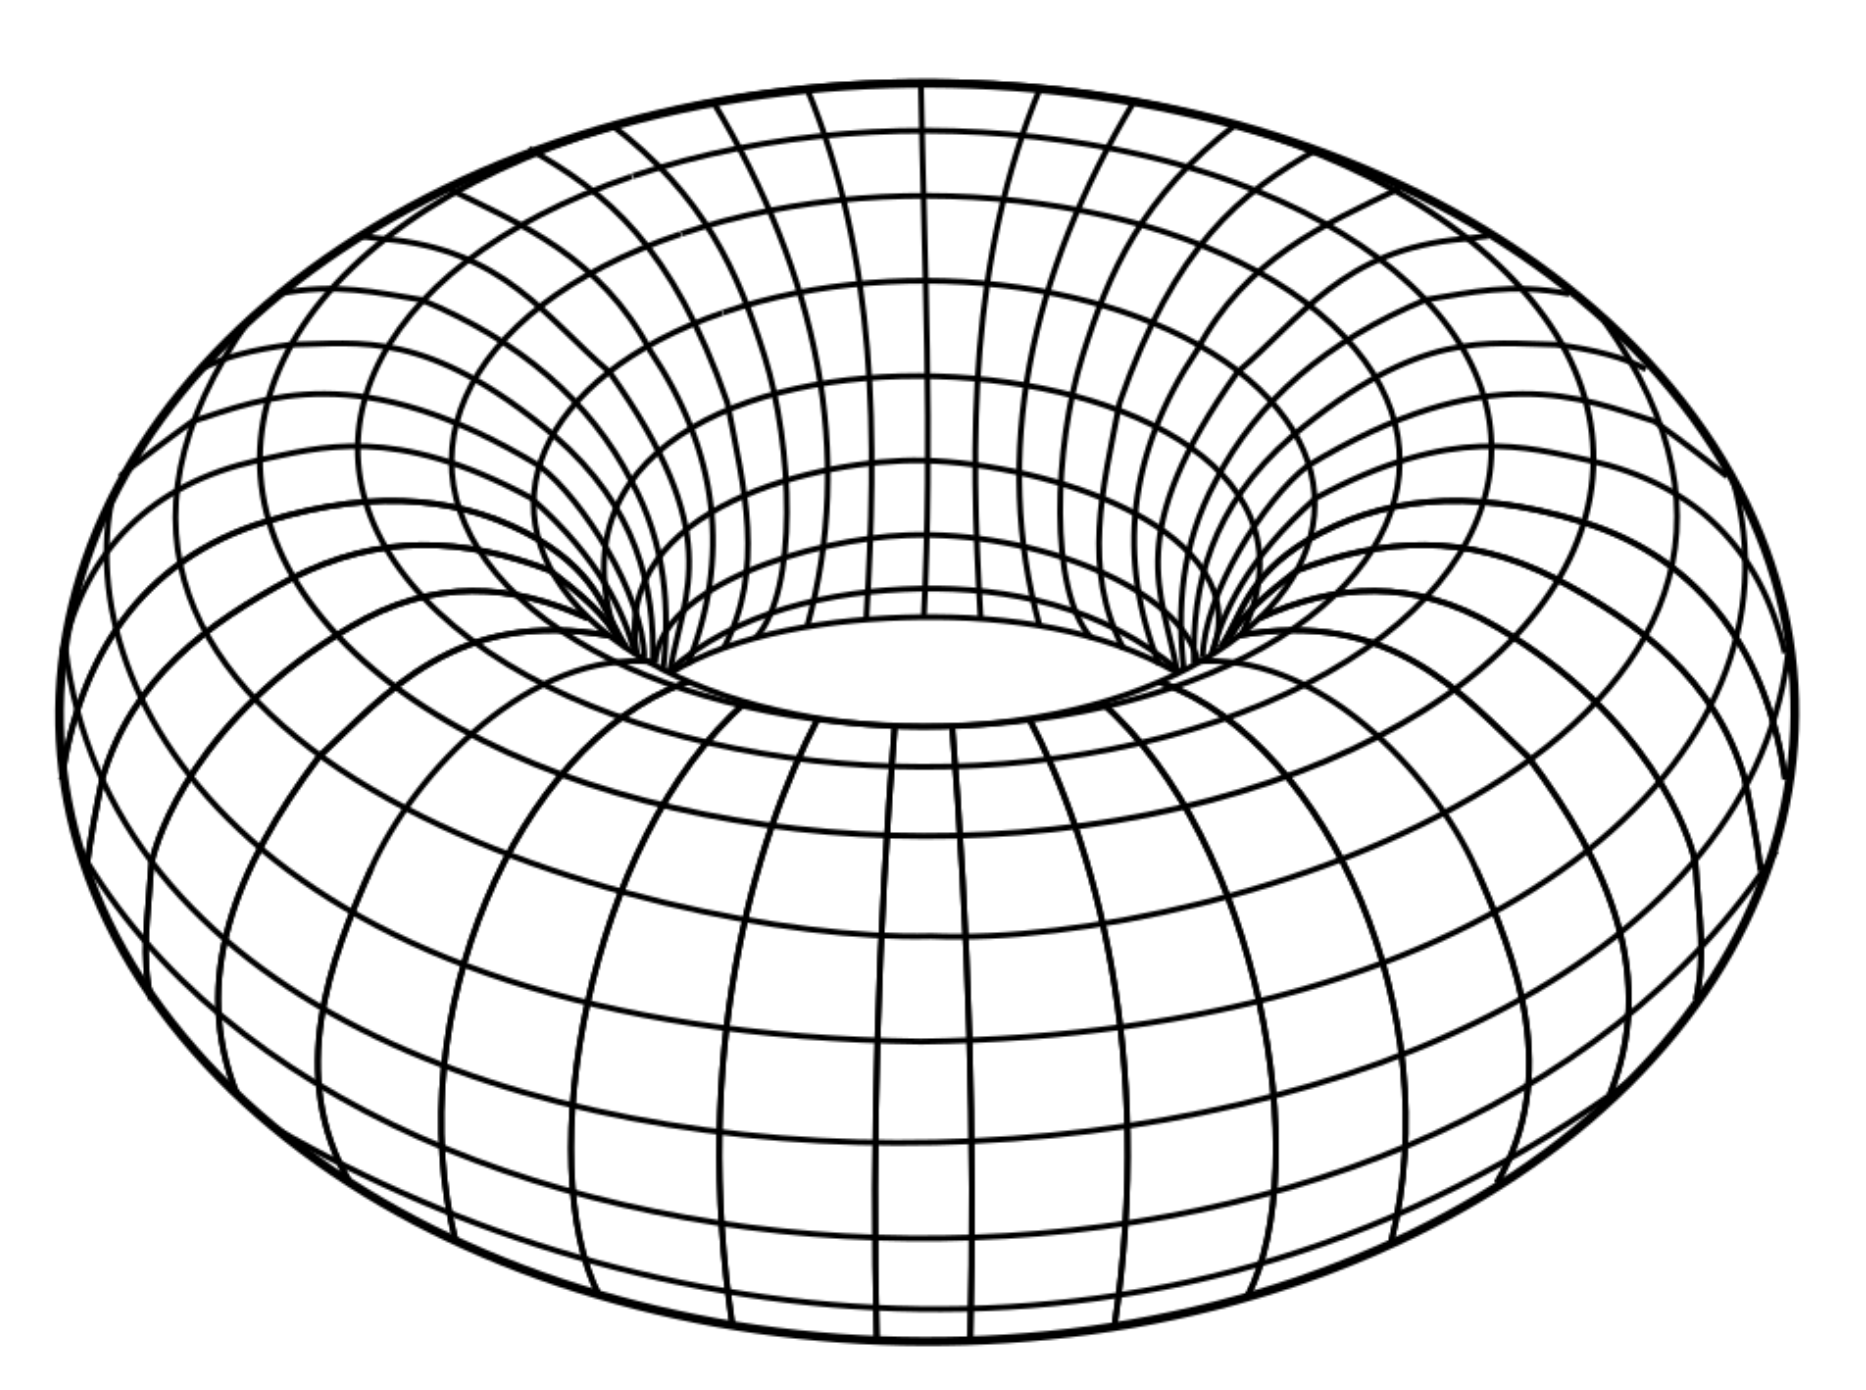
\includegraphics[width=0.7\textwidth]{Pic/Torus.png}
      \end{center}
      \begin{center}
          Image taken from \cite{PBC}
     \end{center}

\end{column}
\end{columns}
\end{frame}


\subsection{Antiferromagnetic}


\begin{frame}{Antiferromagnetic J=-1, T=0}
\begin{columns}
\begin{column}{0.5\textwidth}
    \begin{center}
     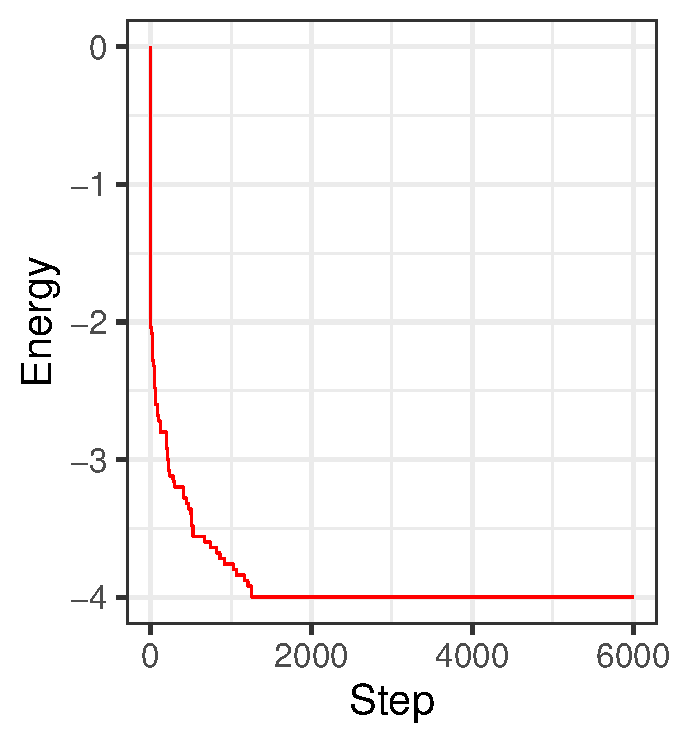
\includegraphics[width=\textwidth]{Pic/J-1_10_6000_T=0_ENERGY.pdf}
     \end{center}
\end{column}
\begin{column}{0.5\textwidth}
    \begin{center}
     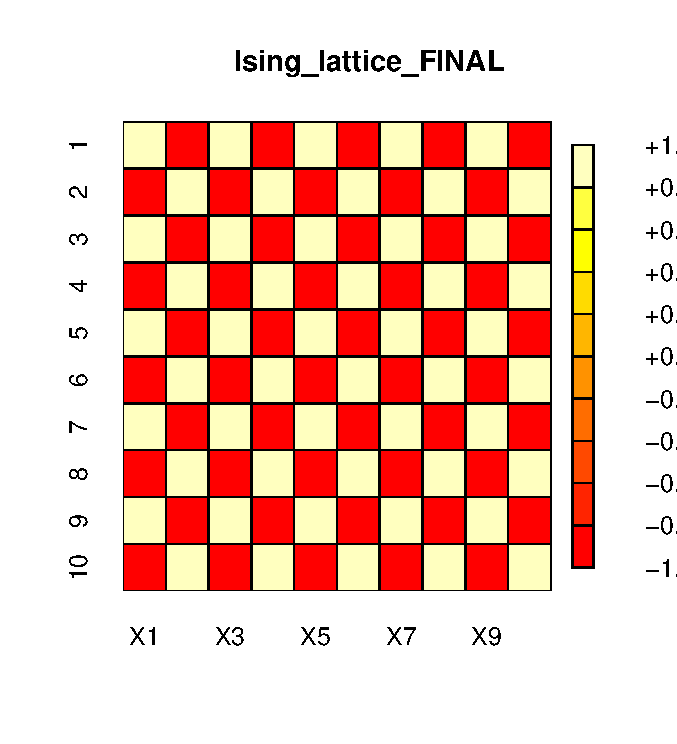
\includegraphics[width=\textwidth]{Pic/J-1_10_6000_T=0_FINAL.pdf}
     \end{center}
\end{column}
\end{columns}
\end{frame}

\begin{frame}{Antiferromagnetic J=-1, T=0}
\begin{columns}
\begin{column}{0.5\textwidth}
    \begin{center}
     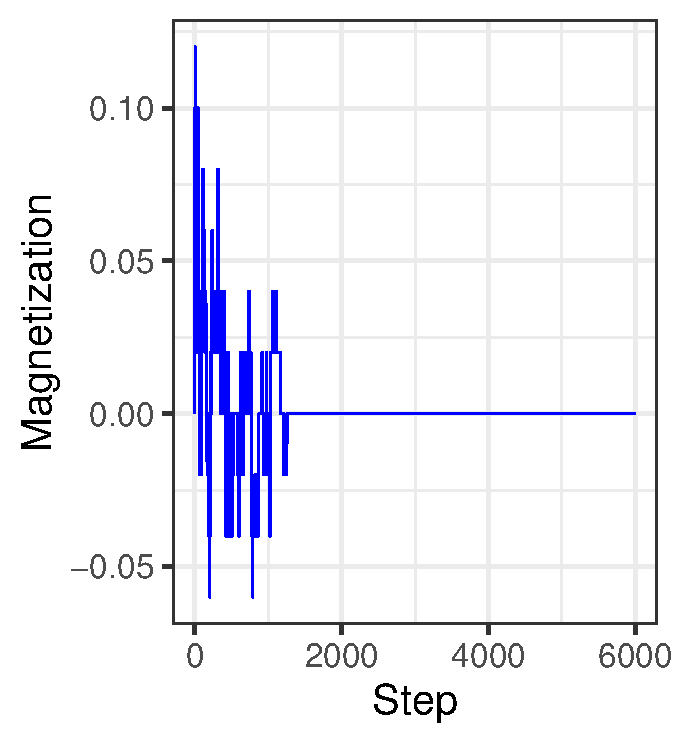
\includegraphics[width=\textwidth]{Pic/J-1_10_6000_T=0_Magnetization.pdf}
     \end{center}
\end{column}
\begin{column}{0.5\textwidth}
    \begin{center}
     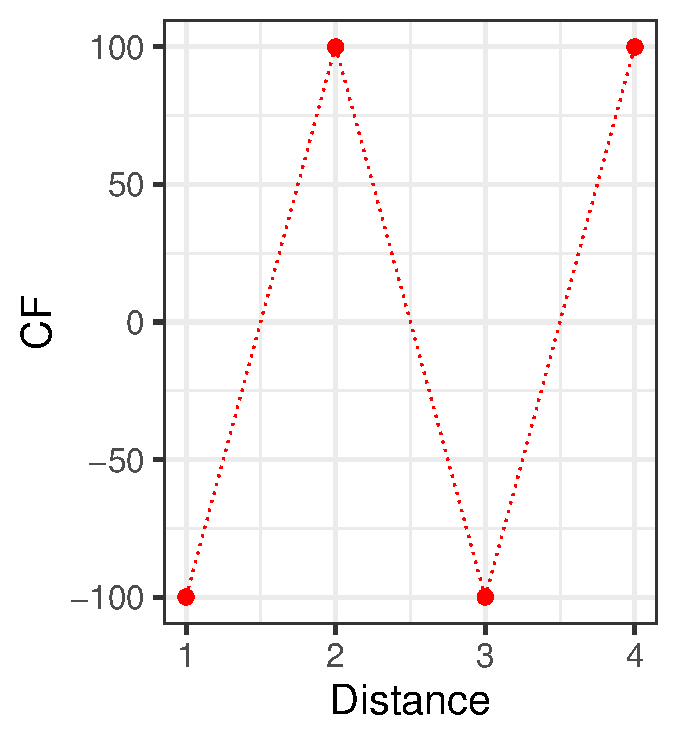
\includegraphics[width=\textwidth]{Pic/J-1_10_6000_T=0_CORRELATION.pdf}
     \end{center}
\end{column}
\end{columns}
\end{frame}


\begin{frame}{Antiferromagnetic J=-1, T=1.5}
\begin{columns}
\begin{column}{0.5\textwidth}
    \begin{center}
     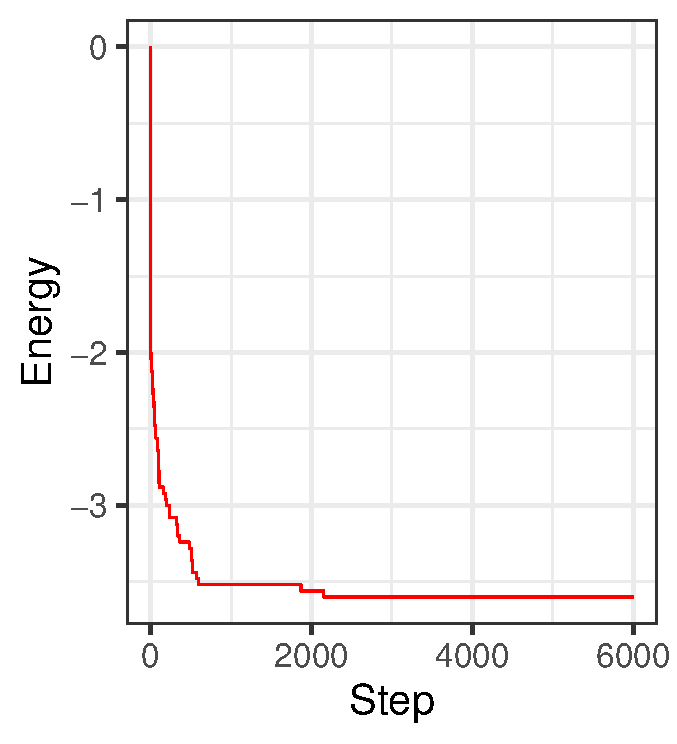
\includegraphics[width=\textwidth]{Pic/J-1_60_2500_T=1.5_ENERGY.pdf}
     \end{center}
\end{column}
\begin{column}{0.5\textwidth}
    \begin{center}
     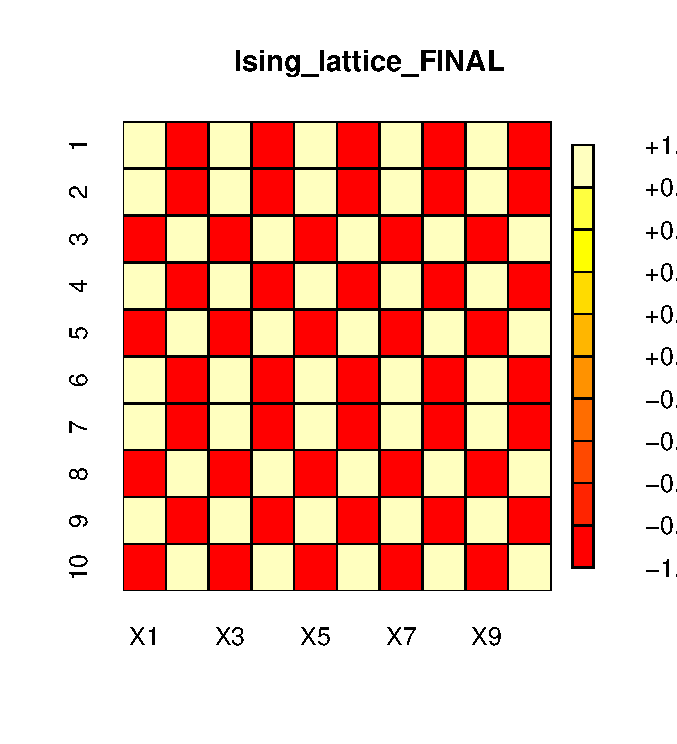
\includegraphics[width=\textwidth]{Pic/J-1_60_2500_T=1.5_FINAL.pdf}
     \end{center}
\end{column}
\end{columns}
\end{frame}

\begin{frame}{Antiferromagnetic J=-1, T=1.5}
\begin{columns}
\begin{column}{0.5\textwidth}
    \begin{center}
     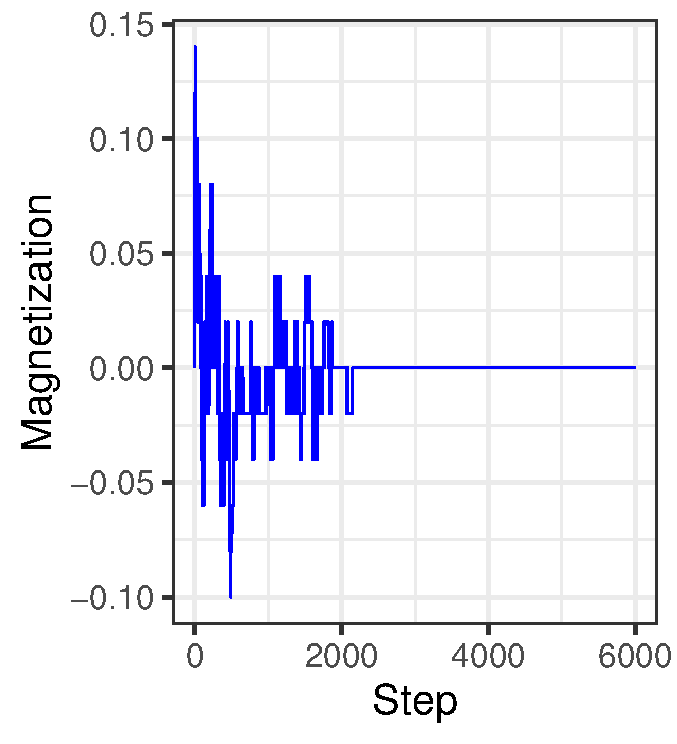
\includegraphics[width=\textwidth]{Pic/J-1_60_2500_T=1.5_Magnetization.pdf}
     \end{center}
\end{column}
\begin{column}{0.5\textwidth}
    \begin{center}
     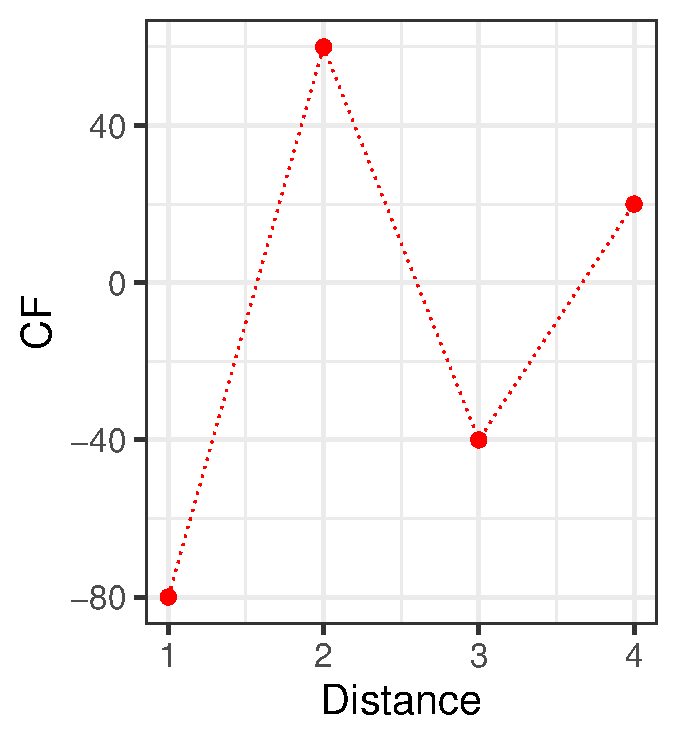
\includegraphics[width=\textwidth]{Pic/J-1_60_2500_T=1.5_CORRELATION.pdf}
     \end{center}
\end{column}
\end{columns}
\end{frame}

\begin{frame}{Antiferromagnetic J=-1, T=4}
\begin{columns}
\begin{column}{0.5\textwidth}
    \begin{center}
     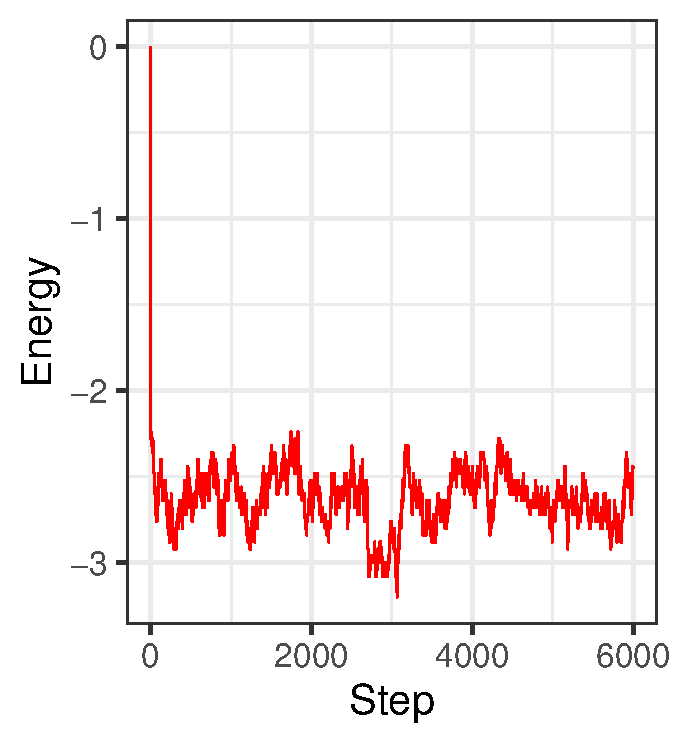
\includegraphics[width=\textwidth]{Pic/J-1_60_2500_T=4_ENERGY.pdf}
     \end{center}
\end{column}
\begin{column}{0.5\textwidth}
    \begin{center}
     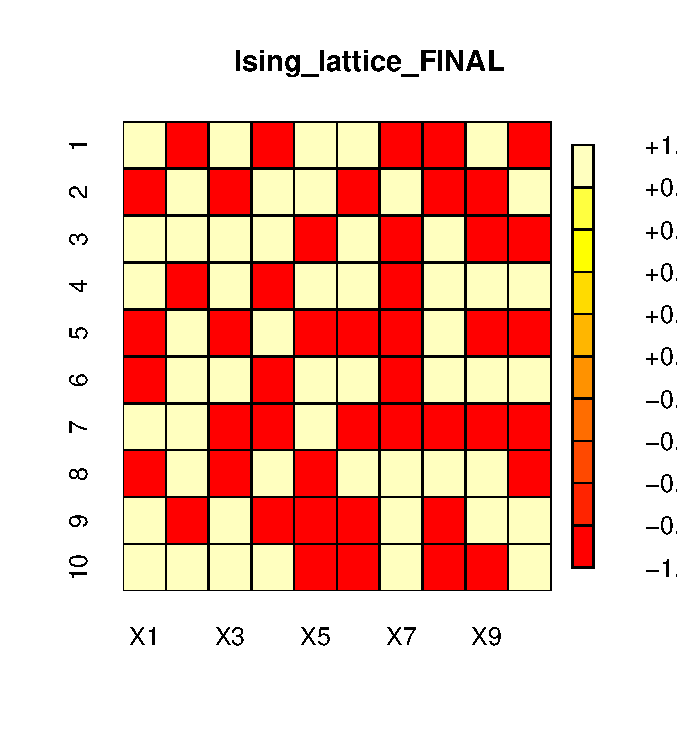
\includegraphics[width=\textwidth]{Pic/J-1_60_2500_T=4_FINAL.pdf}
     \end{center}
\end{column}
\end{columns}
\end{frame}

\begin{frame}{Antiferromagnetic J=-1, T=4}
\begin{columns}
\begin{column}{0.5\textwidth}
    \begin{center}
     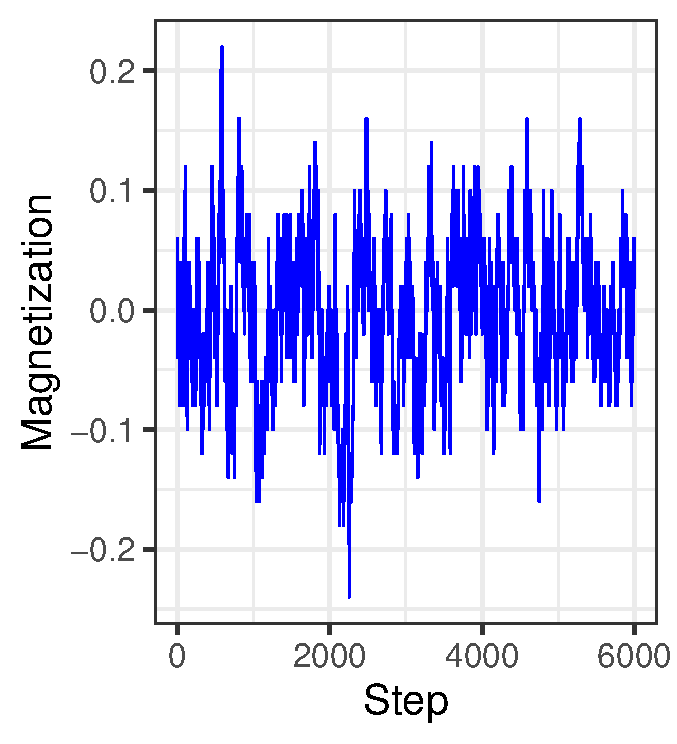
\includegraphics[width=\textwidth]{Pic/J-1_60_2500_T=4_Magnetization.pdf}
     \end{center}
\end{column}
\begin{column}{0.5\textwidth}
    \begin{center}
     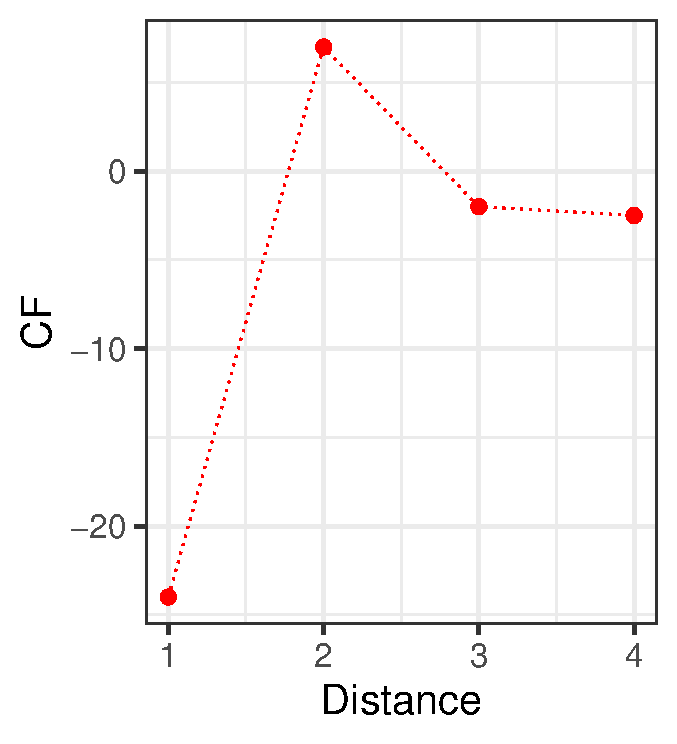
\includegraphics[width=\textwidth]{Pic/J-1_60_2500_T=4_CORRELATION.pdf}
     \end{center}
\end{column}
\end{columns}
\end{frame}


\begin{frame}{Antiferromagnetic J=-1, T=8}
\begin{columns}
\begin{column}{0.5\textwidth}
    \begin{center}
     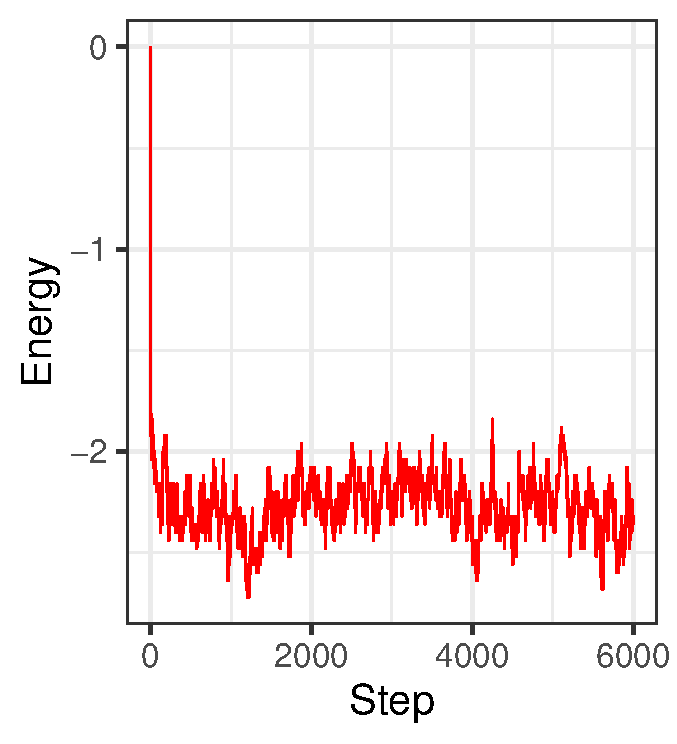
\includegraphics[width=\textwidth]{Pic/J-1_60_2500_T=8_ENERGY.pdf}
     \end{center}
\end{column}
\begin{column}{0.5\textwidth}
    \begin{center}
     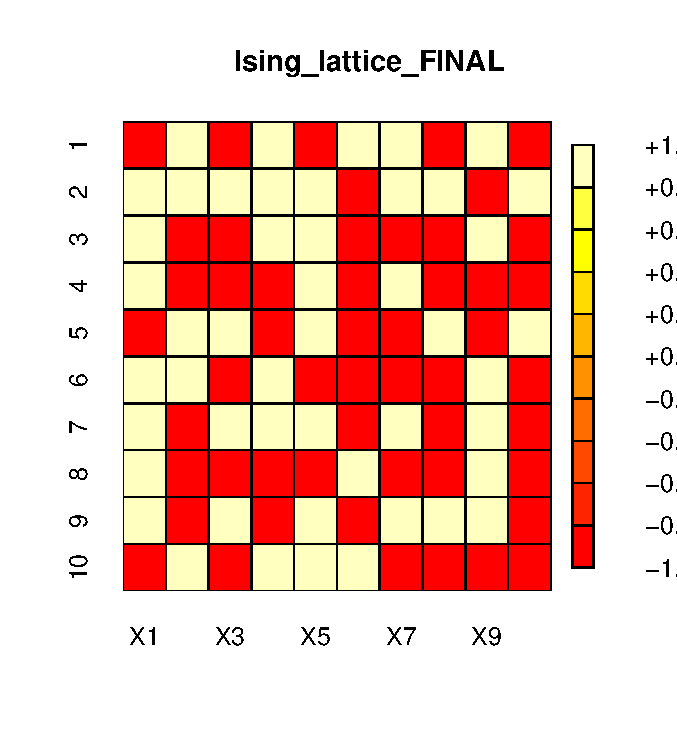
\includegraphics[width=\textwidth]{Pic/J-1_60_2500_T=8_FINAL.pdf}
     \end{center}
\end{column}
\end{columns}
\end{frame}

\begin{frame}{Antiferromagnetic J=-1, T=8}
\begin{columns}
\begin{column}{0.5\textwidth}
    \begin{center}
     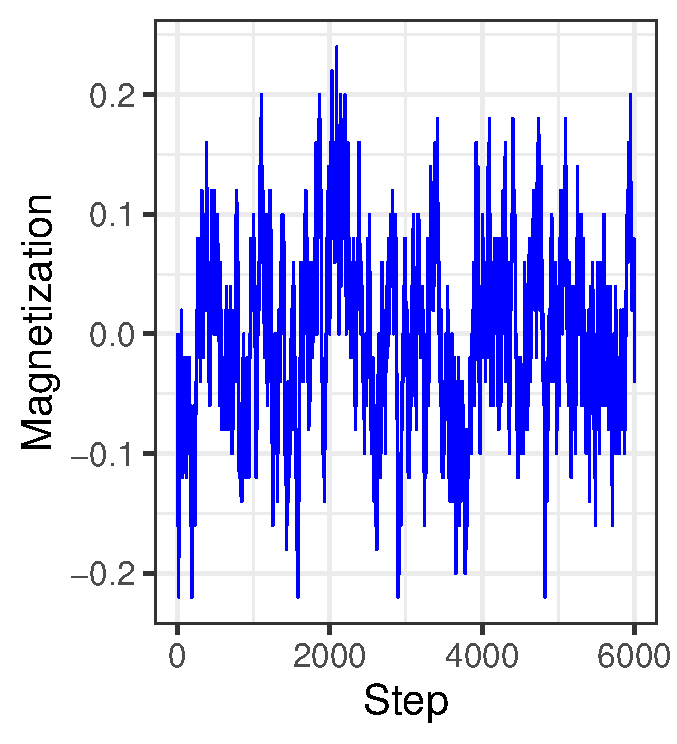
\includegraphics[width=\textwidth]{Pic/J-1_60_2500_T=8_Magnetization.pdf}
     \end{center}
\end{column}
\begin{column}{0.5\textwidth}
    \begin{center}
     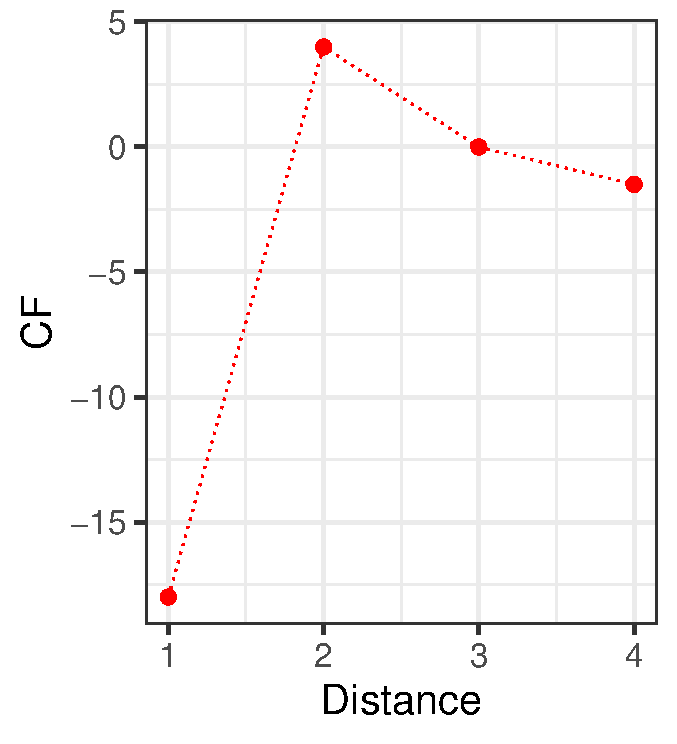
\includegraphics[width=\textwidth]{Pic/J-1_60_2500_T=8_CORRELATION.pdf}
     \end{center}
\end{column}
\end{columns}
\end{frame}

\subsection{Ferromagnetic}

\begin{frame}{Ferromagnetic J=-1, T=30}
\begin{columns}
\begin{column}{0.5\textwidth}
    \begin{center}
     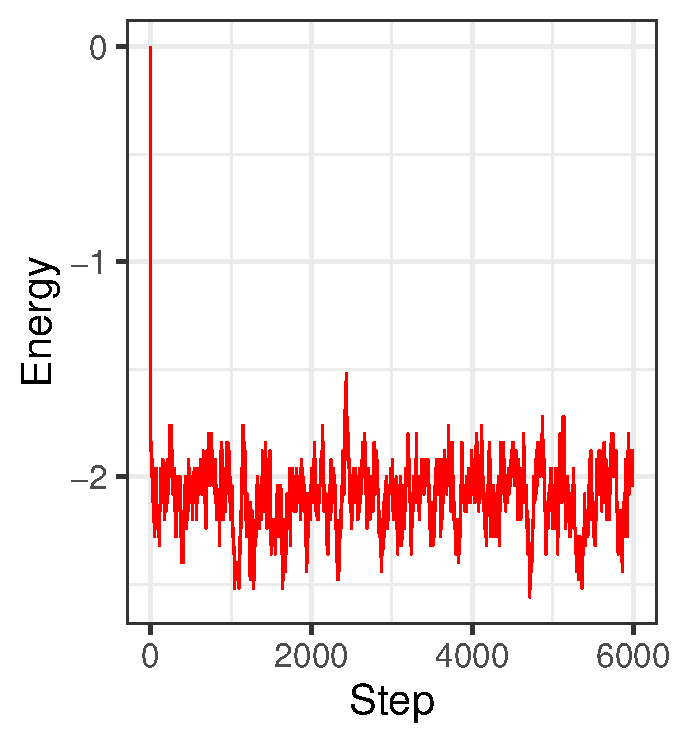
\includegraphics[width=\textwidth]{Pic/J-1_10_6000_T=30_ENERGY.pdf}
     \end{center}
\end{column}
\begin{column}{0.5\textwidth}
    \begin{center}
     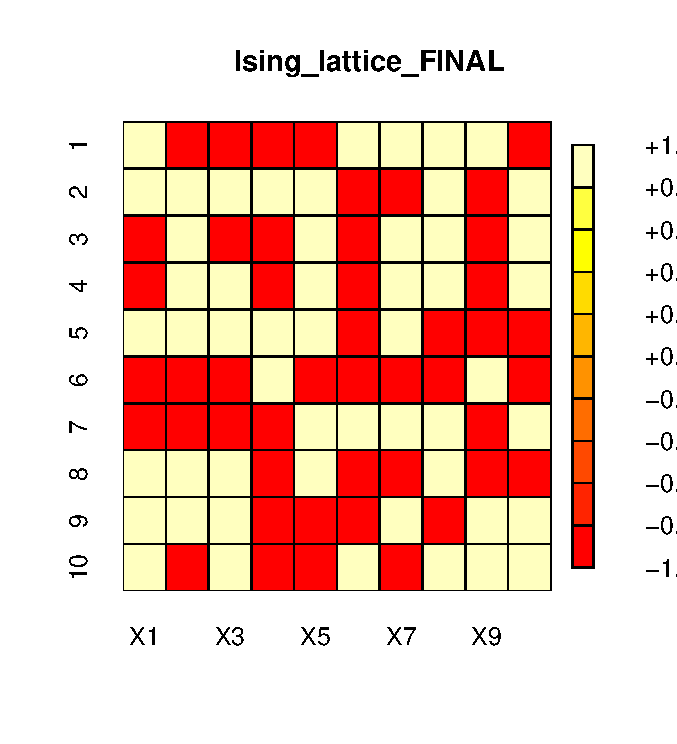
\includegraphics[width=\textwidth]{Pic/J-1_10_6000_T=30_FINAL.pdf}
     \end{center}
\end{column}
\end{columns}
\end{frame}

\begin{frame}{Ferromagnetic J=-1, T=30}
\begin{columns}
\begin{column}{0.5\textwidth}
    \begin{center}
     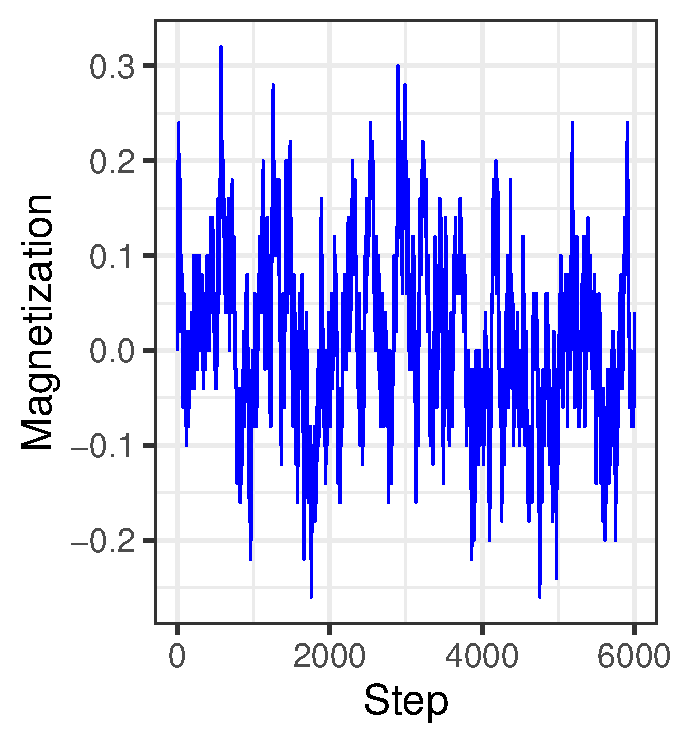
\includegraphics[width=\textwidth]{Pic/J-1_10_6000_T=30_Magnetization.pdf}
     \end{center}
\end{column}
\begin{column}{0.5\textwidth}
    \begin{center}
     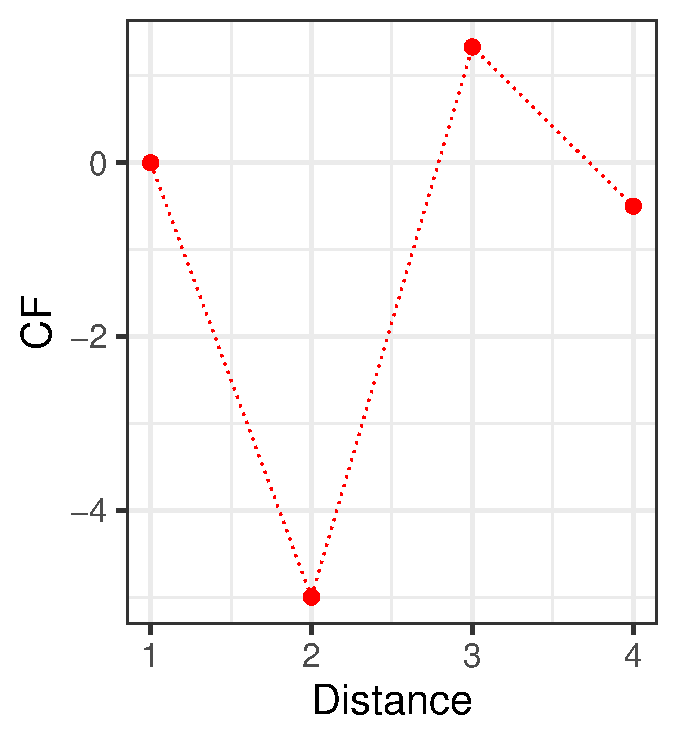
\includegraphics[width=\textwidth]{Pic/J-1_10_6000_T=30_CORRELATION.pdf}
     \end{center}
\end{column}
\end{columns}
\end{frame}

\begin{frame}{Ferromagnetic J=+1, T=0}
\begin{columns}
\begin{column}{0.5\textwidth}
    \begin{center}
     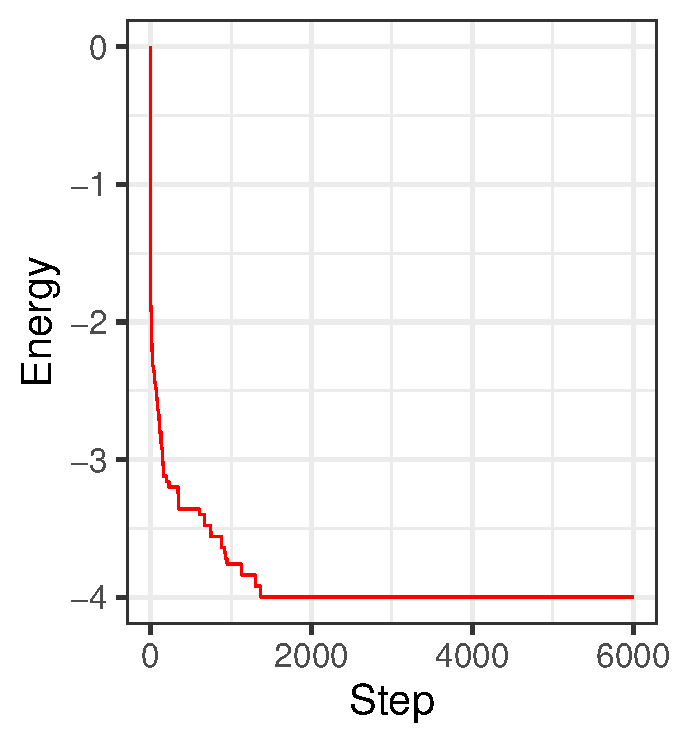
\includegraphics[width=\textwidth]{Pic/J+1_10_6000_T=0_ENERGY.pdf}
     \end{center}
\end{column}
\begin{column}{0.5\textwidth}
    \begin{center}
     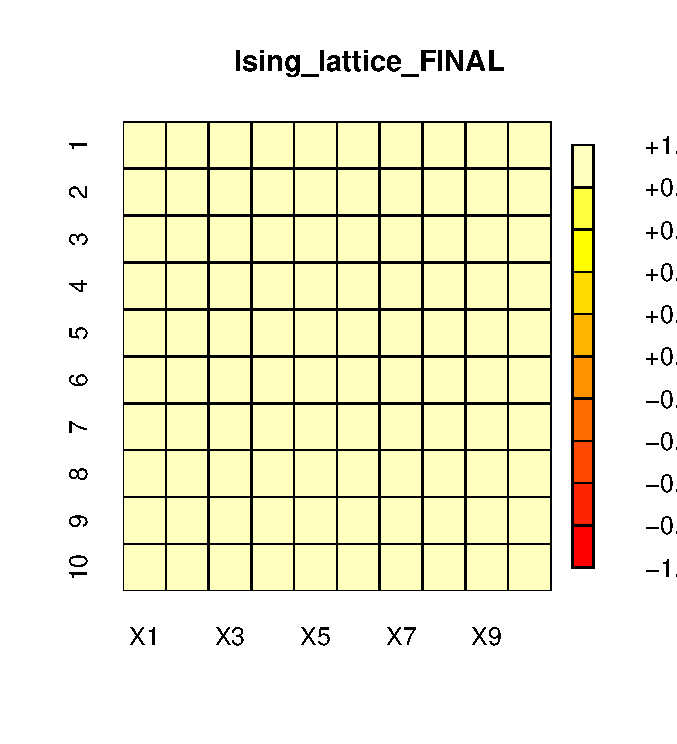
\includegraphics[width=\textwidth]{Pic/J+1_10_6000_T=0_FINAL.pdf}
     \end{center}
\end{column}
\end{columns}
\end{frame}

\begin{frame}{Ferromagnetic J=+1, T=0}
\begin{columns}
\begin{column}{0.5\textwidth}
    \begin{center}
     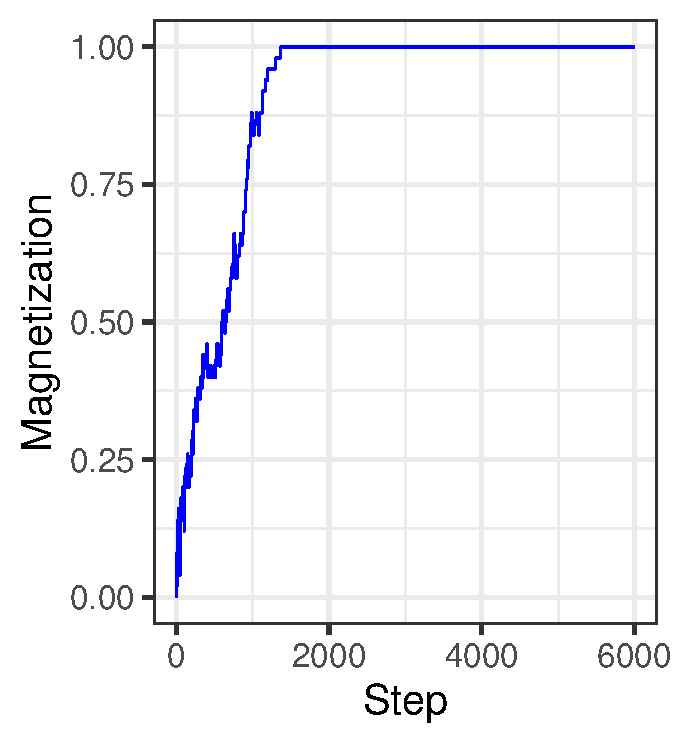
\includegraphics[width=\textwidth]{Pic/J+1_10_6000_T=0_Magnetization.pdf}
     \end{center}
\end{column}
\begin{column}{0.5\textwidth}
    \begin{center}
     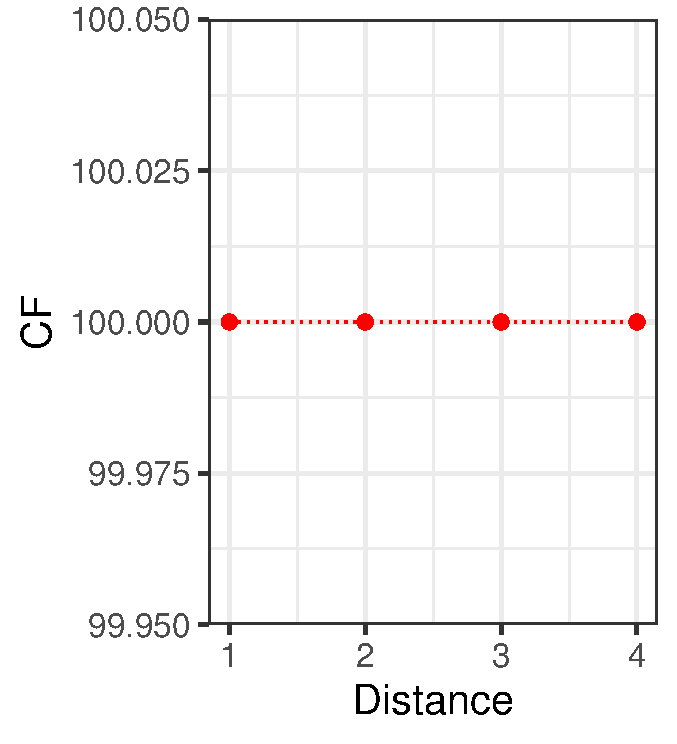
\includegraphics[width=\textwidth]{Pic/J+1_10_6000_T=0_Coherence.pdf}
     \end{center}
\end{column}
\end{columns}
\end{frame}

\begin{frame}{Ferromagnetic J=+1, T=8}
\begin{columns}
\begin{column}{0.5\textwidth}
    \begin{center}
     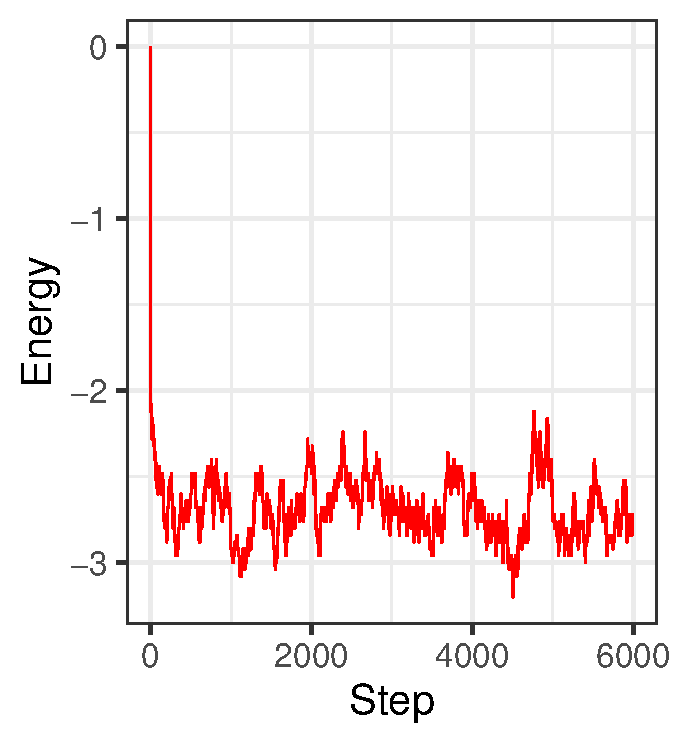
\includegraphics[width=\textwidth]{Pic/J+1_10_6000_T=8_ENERGY.pdf}
     \end{center}
\end{column}
\begin{column}{0.5\textwidth}
    \begin{center}
     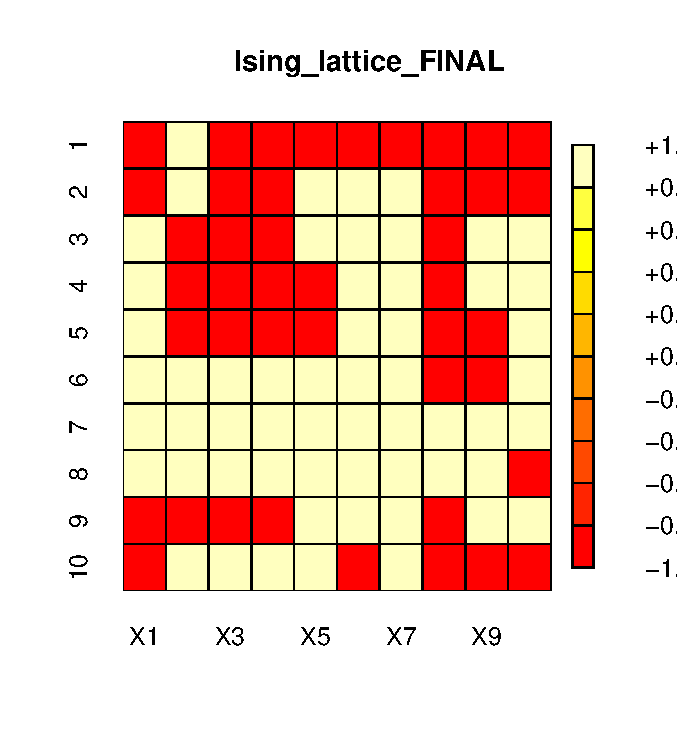
\includegraphics[width=\textwidth]{Pic/J+1_10_6000_T=8_FINAL.pdf}
     \end{center}
\end{column}
\end{columns}
\end{frame}

\begin{frame}{Ferromagnetic J=+1, T=8}
\begin{columns}
\begin{column}{0.5\textwidth}
    \begin{center}
     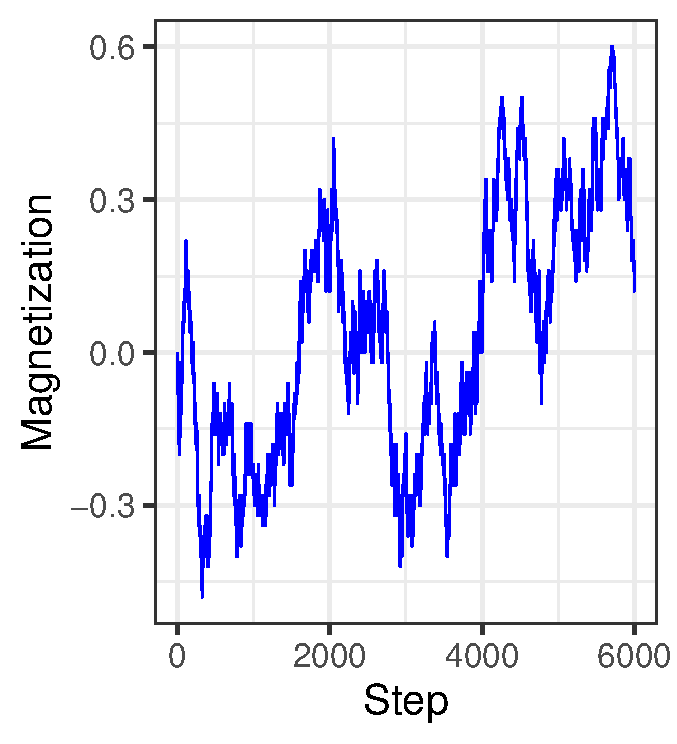
\includegraphics[width=\textwidth]{Pic/J+1_10_6000_T=8_Magnetization.pdf}
     \end{center}
\end{column}
\begin{column}{0.5\textwidth}
    \begin{center}
     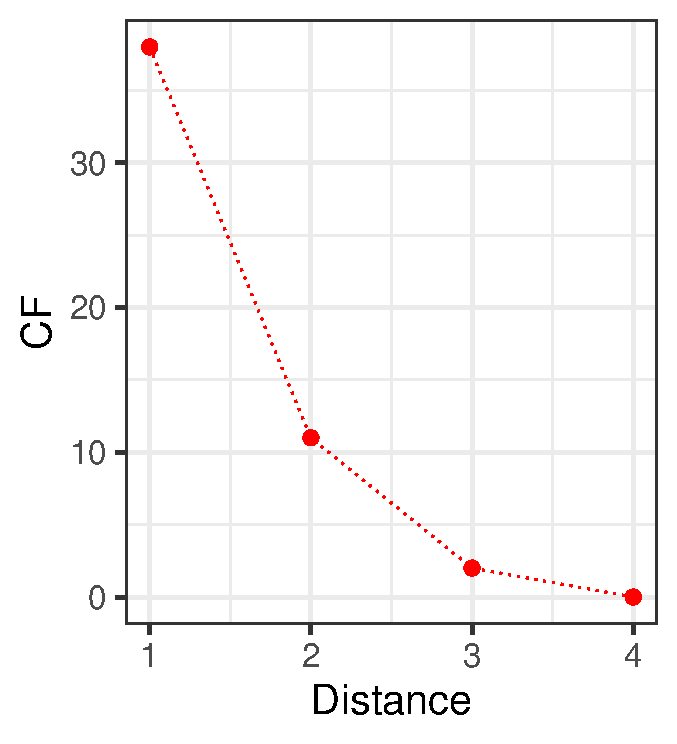
\includegraphics[width=\textwidth]{Pic/J+1_10_6000_T=8_Coherence.pdf}
     \end{center}
\end{column}
\end{columns}
\end{frame}

\begin{frame}{Ferromagnetic J=+1, T=16}
\begin{columns}
\begin{column}{0.5\textwidth}
    \begin{center}
     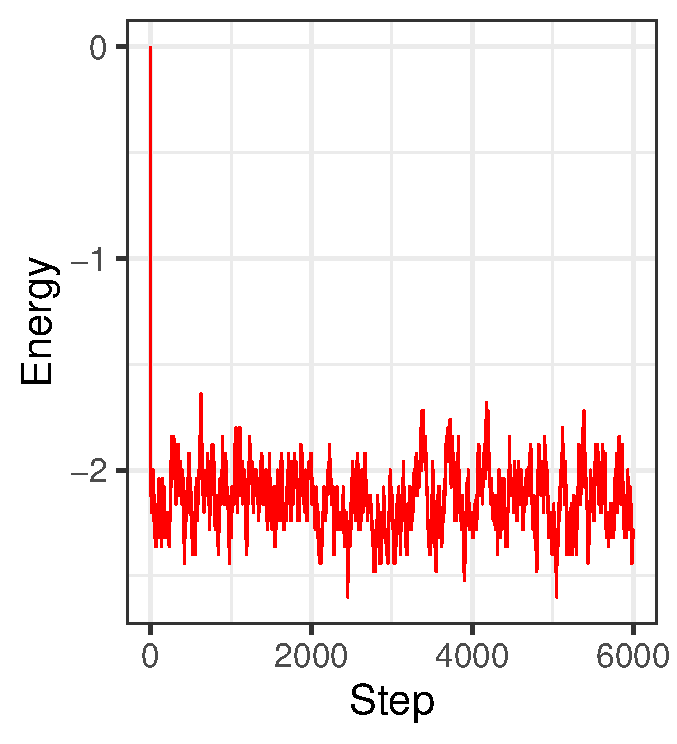
\includegraphics[width=\textwidth]{Pic/J+1_10_2500_T=16_ENERGY.pdf}
     \end{center}
\end{column}
\begin{column}{0.5\textwidth}
    \begin{center}
     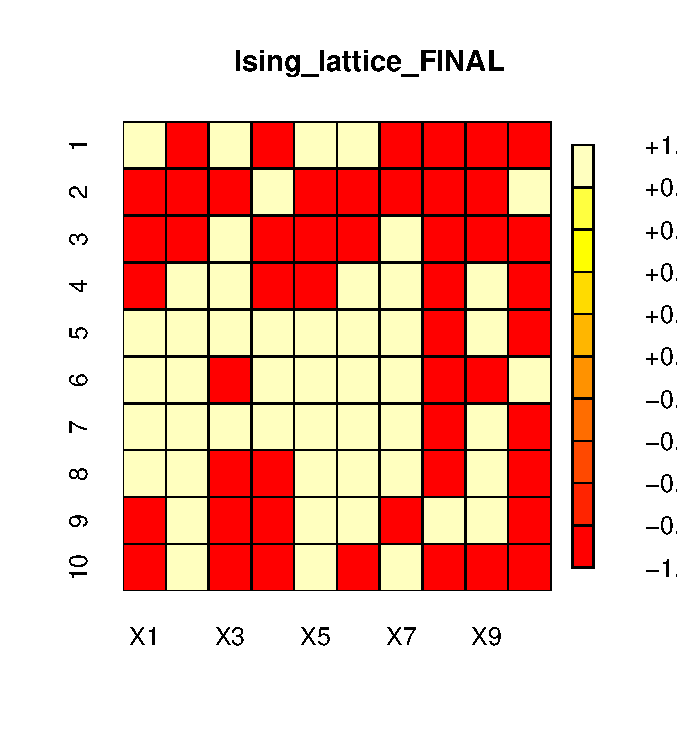
\includegraphics[width=\textwidth]{Pic/J+1_10_2500_T=16_FINAL.pdf}
     \end{center}
\end{column}
\end{columns}
\end{frame}

\begin{frame}{Ferromagnetic J=+1, T=16}
\begin{columns}
\begin{column}{0.5\textwidth}
    \begin{center}
     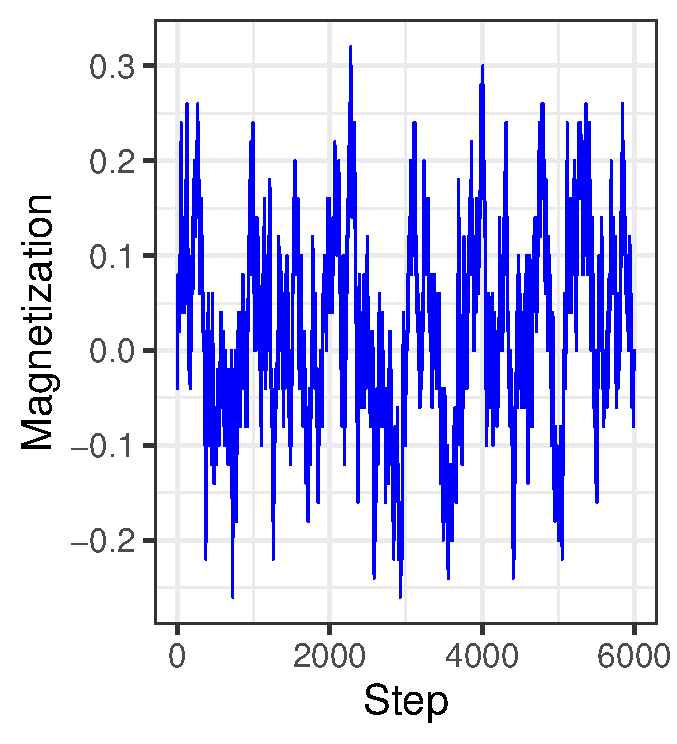
\includegraphics[width=\textwidth]{Pic/J+1_10_2500_T=16_Magnetization.pdf}
     \end{center}
\end{column}
\begin{column}{0.5\textwidth}
    \begin{center}
     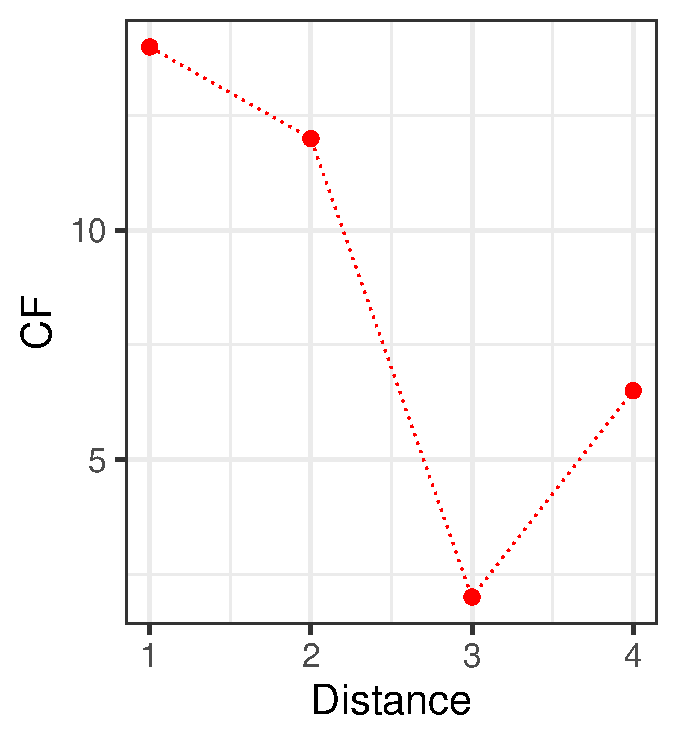
\includegraphics[width=\textwidth]{Pic/J+1_10_2500_T=16_Coherence.pdf}
     \end{center}
\end{column}
\end{columns}
\end{frame}



\begin{frame}{Ferromagnetic with two centers T=0}
    \begin{center}
     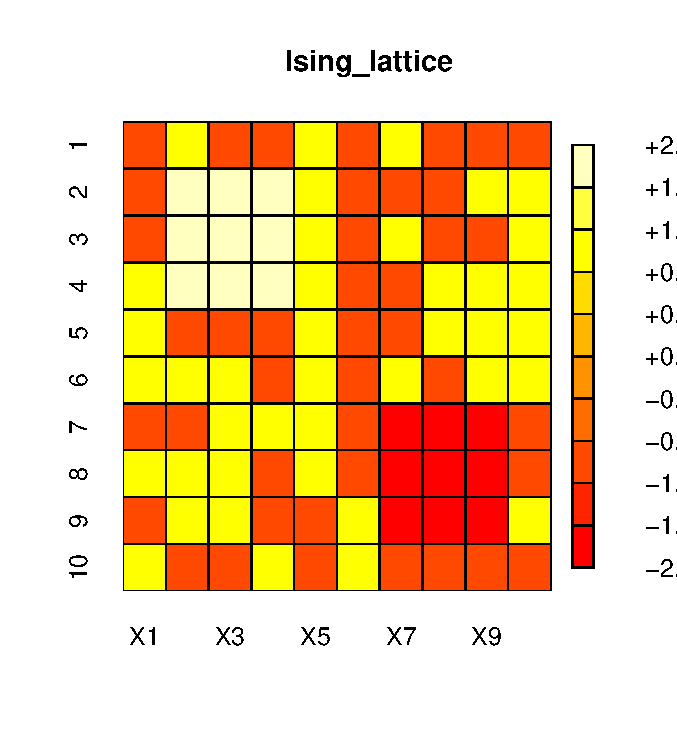
\includegraphics[width=0.5\textwidth]{Pic/2CENTER.pdf}
     \end{center}
\end{frame}


\begin{frame}{Ferromagnetic with two centers T=0}
\begin{columns}
\begin{column}{0.5\textwidth}
    \begin{center}
     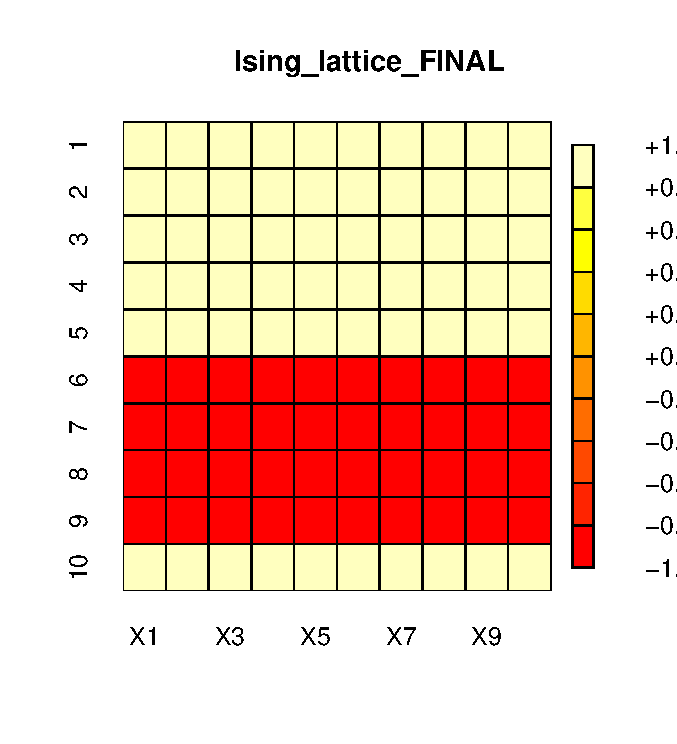
\includegraphics[width=\textwidth]{Pic/J+1_10_6000_two_center_T=0_FINAL.pdf}
     \end{center}
\end{column}
\begin{column}{0.5\textwidth}
    \begin{center}
     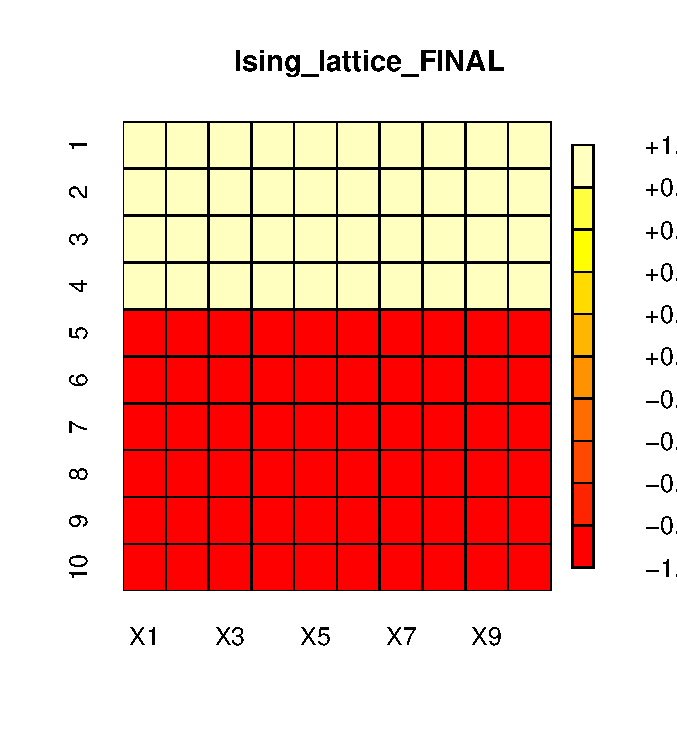
\includegraphics[width=\textwidth]{Pic/J+1_10_6000_two_center_T=0_2_FINAL.pdf}
     \end{center}
\end{column}
\end{columns}
\end{frame}


\begin{frame}{Ferromagnetic with two centers T=0, 20$\times$20}
    \begin{center}
     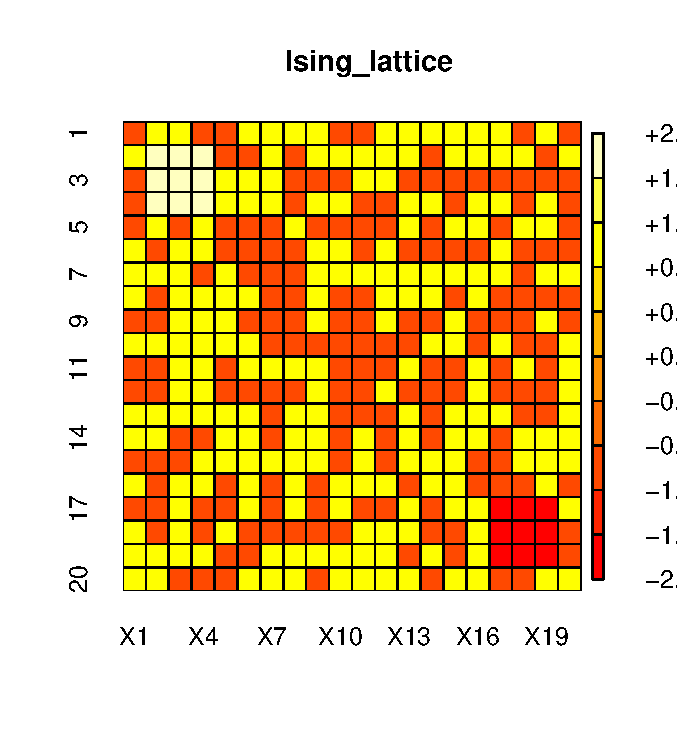
\includegraphics[width=0.5\textwidth]{Pic/LATTICE20x20TWOCENTER.pdf}
     \end{center}
\end{frame}

\begin{frame}{Ferromagnetic with two centers T=0,  20$\times$20}
\begin{columns}
\begin{column}{0.5\textwidth}
    \begin{center}
     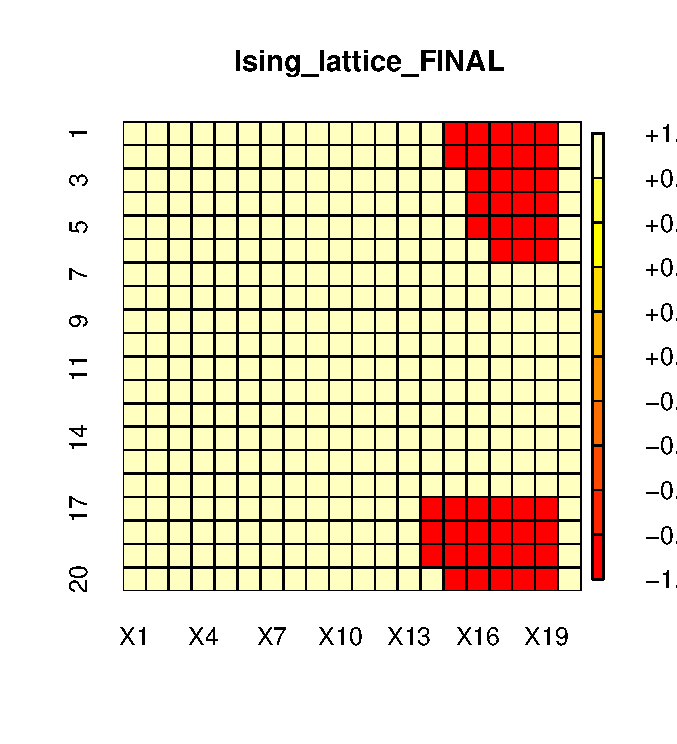
\includegraphics[width=\textwidth]{Pic/J+1_20_10000_T=0_FINAL.pdf}
     \end{center}
\end{column}
\begin{column}{0.5\textwidth}
    \begin{center}
     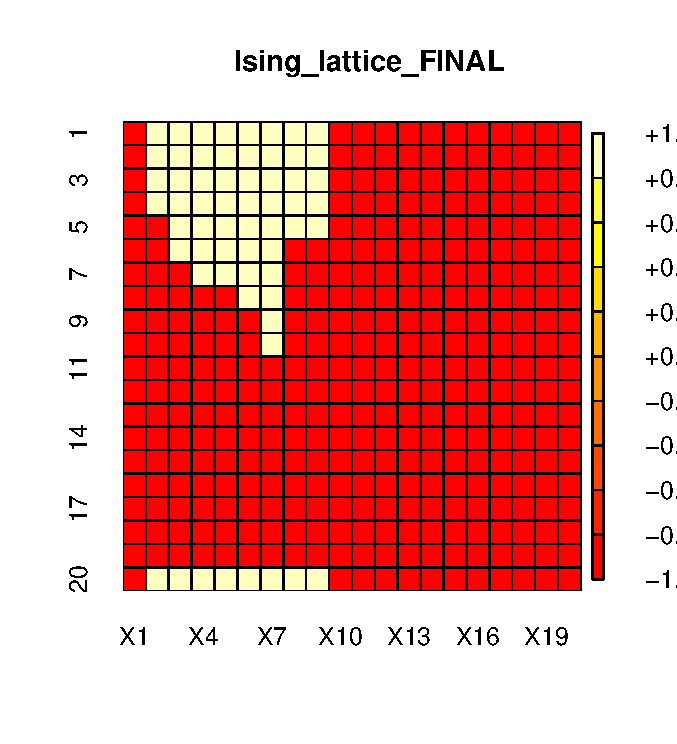
\includegraphics[width=\textwidth]{Pic/J+1_20_10000_T=0_FINAL_2.pdf}
     \end{center}
\end{column}
\end{columns}
\end{frame}

\begin{frame}{Ferromagnetic with two centers T=0.25,  20$\times$20}
\begin{columns}
\begin{column}{0.5\textwidth}
    \begin{center}
     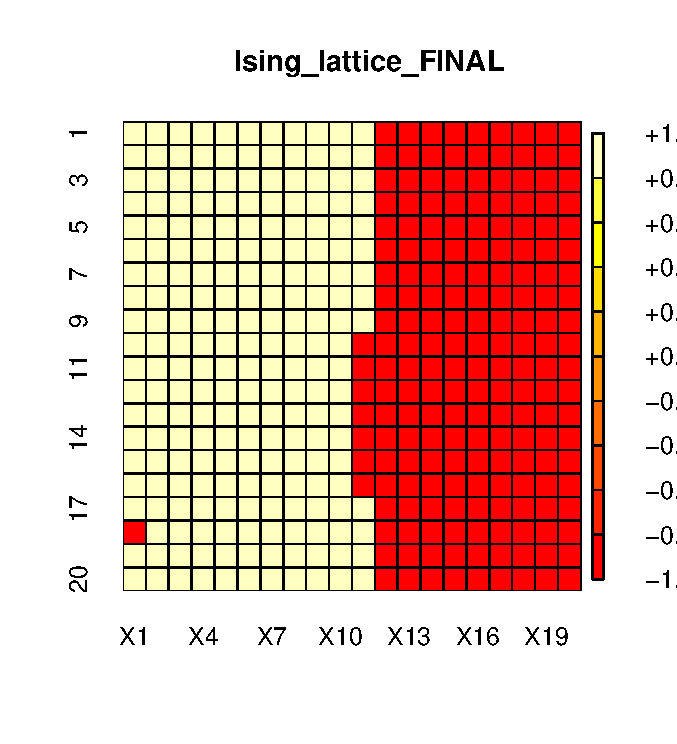
\includegraphics[width=\textwidth]{Pic/J+1_20_10000_T=0.25.pdf}
     \end{center}
\end{column}
\begin{column}{0.5\textwidth}
    \begin{center}
     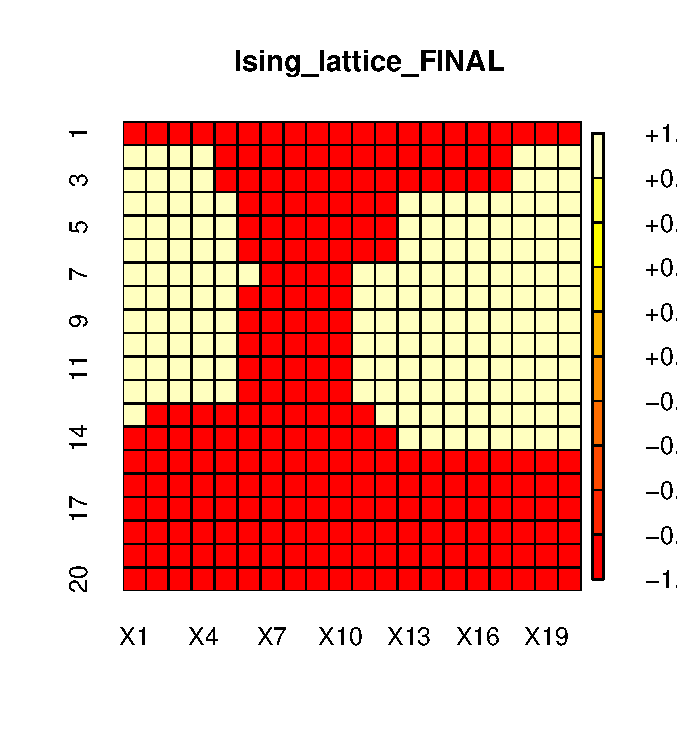
\includegraphics[width=\textwidth]{Pic/J+1_20_10000_T=0.25_2.pdf}
     \end{center}
\end{column}
\end{columns}
\end{frame}

\begin{frame}{Ferromagnetic with two centers T=0,  60$\times$60}
\begin{columns}
\begin{column}{0.5\textwidth}
    \begin{center}
     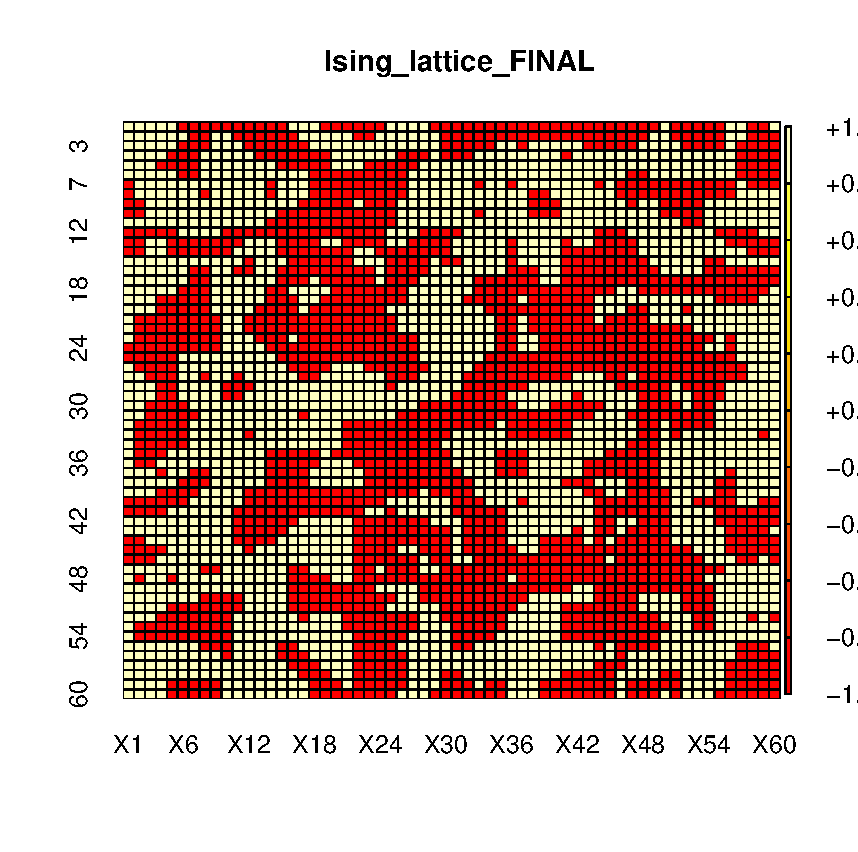
\includegraphics[width=\textwidth]{Pic/J+1_60_10000_T=0_FINAL.pdf}
     \end{center}
\end{column}
\begin{column}{0.5\textwidth}
    \begin{center}
     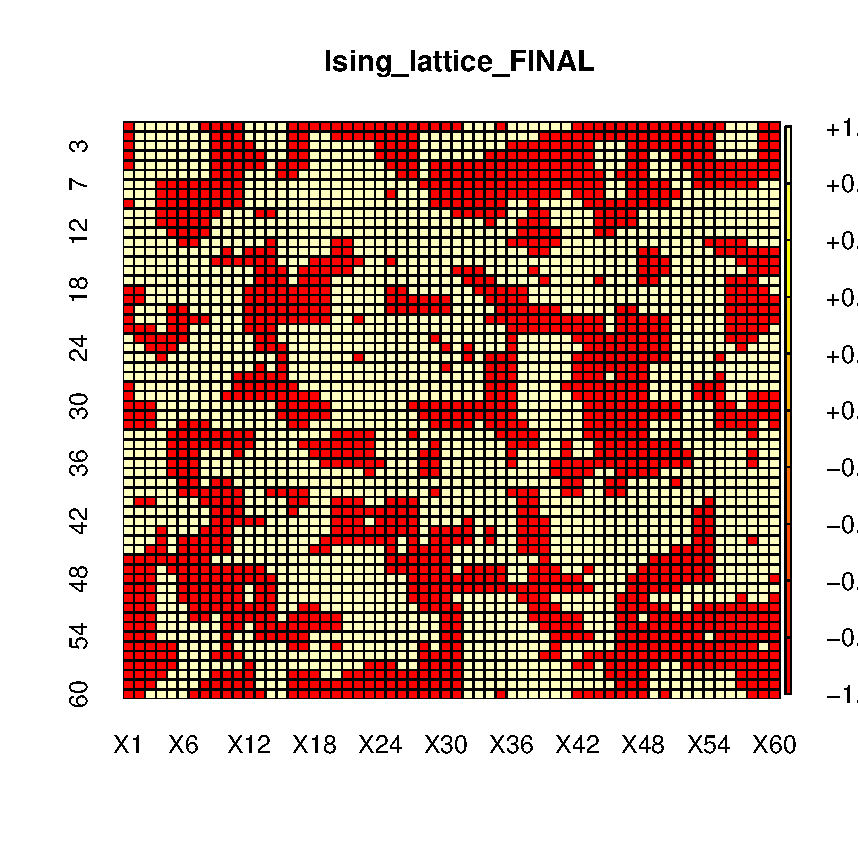
\includegraphics[width=\textwidth]{Pic/J+1_60_10000_T=0_2_FINAL.pdf}
     \end{center}
\end{column}
\end{columns}
\end{frame}

\begin{frame}{Ferromagnetic with two centers $T>0$,  60$\times$60}
\begin{columns}
\begin{column}{0.3\textwidth}
    \begin{center}
     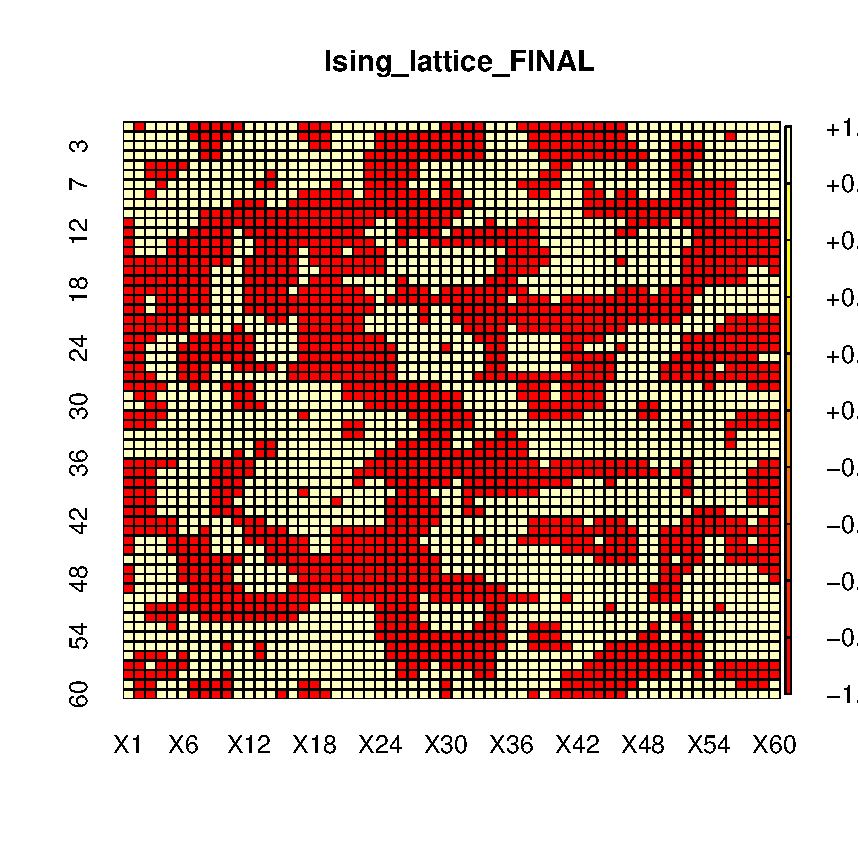
\includegraphics[width=\textwidth]{Pic/J+1_60_10000_T=1_FINAL.pdf}
     \end{center}
         \begin{center}
     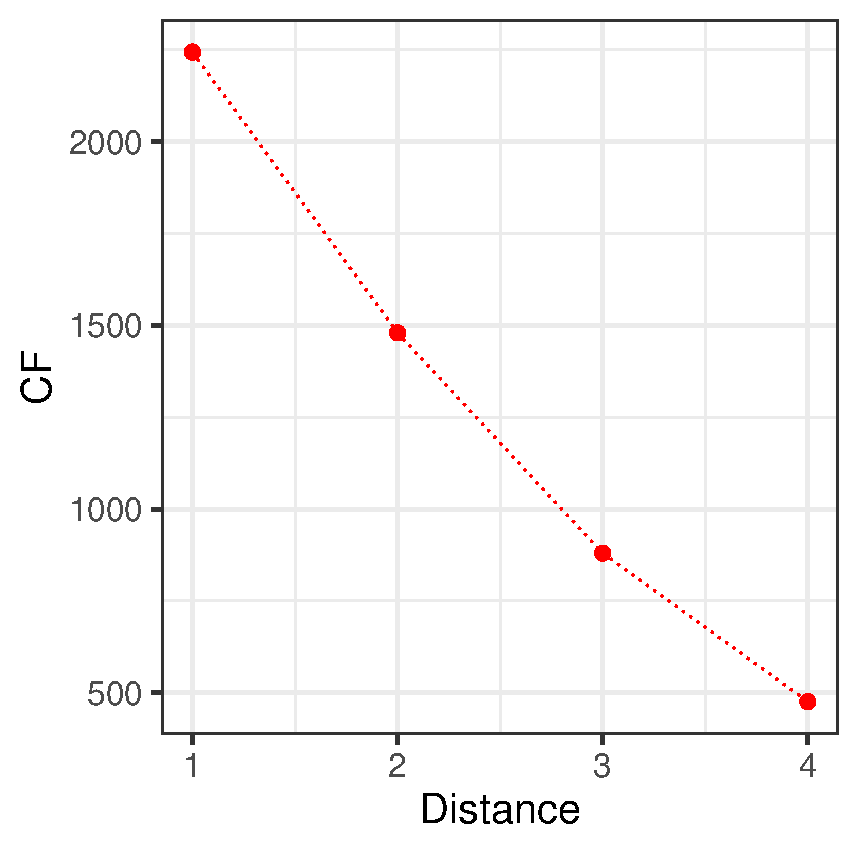
\includegraphics[width=\textwidth]{Pic/J+1_60_10000_T=1_FINAL_COHERENCE.pdf}
     \end{center}
\end{column}
\begin{column}{0.3\textwidth}
    \begin{center}
     \includegraphics[width=\textwidth]{Pic/J+1_60_10000_T=4_FINAL.pdf}
     \end{center}
 
              \begin{center}
     \includegraphics[width=\textwidth]{Pic/J+1_60_10000_T=4_FINAL_COHERENCE.pdf}
     \end{center}
\end{column}
\begin{column}{0.3\textwidth}
    \begin{center}
     \includegraphics[width=\textwidth]{Pic/J+1_60_10000_T=8_FINAL.pdf}
     \end{center}
         \begin{center}
     \includegraphics[width=\textwidth]{Pic/J+1_60_10000_T=8_COHERENCE.pdf}
     \end{center}
\end{column}
\end{columns}
\end{frame}


\begin{frame}{Ferromagnetic with four centers T=0,  60$\times$60}
    \begin{center}
     \includegraphics[width=0.6\textwidth]{Pic/J+1_60_10000_four_center_T=0_START.pdf}
     \end{center}
\end{frame}


\begin{frame}{Ferromagnetic with two centers T=0,  60$\times$60}
\begin{columns}
\begin{column}{0.5\textwidth}
    \begin{center}
     \includegraphics[width=\textwidth]{Pic/J+1_60_10000_four_center_T=0_FINAL.pdf}
     \end{center}
\end{column}
\begin{column}{0.5\textwidth}
    \begin{center}
     \includegraphics[width=\textwidth]{Pic/J+1_60_10000_T=0_2_FINAL.pdf}
     \end{center}
\end{column}
\end{columns}
\end{frame}



\begin{frame}[t,allowframebreaks]
\frametitle{Bibliography}
\printbibliography
\end{frame}



\section{Supporting Info}




\begin{frame}{Concepts of statistical mechanics: entropy \cite{peliti2011statistical}}
\textbf{Central problem of thermodynamics:} characterize the actual state of equilibrium among all virtual states  \\
\textbf{Entropy postulate}: there exist a function S of the extensive variables $(X_{0},X_{1}...X_{r})$ called entropy,  that assumes the maximum value for a state of equilibrium among all vritual states and that possesses the following properties:
\begin{itemize}
\item Extensivity $S^{(1\cup2)}=S^{1}+S^{2}$
\item Convexity $S((1-\alpha)X^{1}+\alpha X^{2}) \geq (1-\alpha)S(x^{1})+\alpha S(X^{2})$
\item Monotonicity $\dfrac{\partial S}{\partial E}|_{X_{1}...X_{r}}=\frac{1}{T}>0$
\end{itemize}
\textbf The equilibrium state corresponds to the maximum entropy compatible with the constrains

\end{frame}


\begin{frame}{Concepts of statistical mechanics: entropy \cite{peliti2011statistical}}

\begin{itemize}
\item \textbf{Fundamental postulate of statistical mechanics} $S=k_{b}\ln|\Gamma|$ Where S is the thermodynamic entropy,  $k_{b}$ is Boltzmann constant and $|\Gamma|$ the volume in the phase space
\end{itemize}
\end{frame}

\end{document}
